\chapter{Simulaciones}
\lhead{\emph{Simulaciones}}

\todo[inline]{Aca vienen las simulaciones y resultados obtenidos de las simulaciones realizadas con el modelo de la antena}
\section{Modelo de la antena}

\todo{agregar el grafico de la composicion de una antena}



\subsection{Configuraciones del sistema}

Las configuraciones que se le pueden realizar al modelo de antena para realizar los distintos ensayos están listados en la 
tabla \ref{tab:conf_modelo_antena1}.

\begin{center}
  \footnotesize
  \centering
  \begin{longtable}{|c|p{9cm}|}
    \hline 
	\multicolumn{2}{|c|}{\textbf{Parámetros de entrada}} \\ 
	\hline
    Frequencia		& Es la frecuenia central de trabajo en Hz \tabularnewline \hline 
    Potencia		& Potencia con la que se alimenta la antena en db \tabularnewline \hline 
    Fase			& Fase con la que se alimenta la antena en grados \tabularnewline \hline 
    Row Steering	& Apuntamiento horizontal que se le quiere dar al beam de salida, en grados  \tabularnewline \hline 
    Column Steering	& Apuntamiento vertical que se le quiere dar al beam de salida, en grados  \tabularnewline \hline 
	\multicolumn{2}{|c|}{\textbf{Parámetros de calibración}} \\ 
	\hline
	potencia Tx deseada	& Potencia de transmisión deseada para calbirar  \tabularnewline \hline 
	potencia Rx deseada	& Potencia de recepción deseada para calbirar  \tabularnewline \hline 
	Errores	& Son los errores referentes a la hora de calibrar el modelo de antena. Pueden ser: interPulseGainChirpError, interPulsePhaseChirpError, gainChirpRepError, phaseChirpRepError, WalPhaseErrors  \tabularnewline \hline
	\multicolumn{2}{|c|}{\textbf{Parámetros de Antena}} \\ 
	\hline
	Cantidad Filas	& Da la cantidad de módulos radiantes en dirección vertical \tabularnewline \hline 
	Cantidad Columnas	& Da la cantidad de módulos radiantes en dirección horizontal \tabularnewline \hline 
	Separación vertical & Es la separación vertical entre RMs \tabularnewline \hline 
	Separación horizontal & Es la separación horizontal entre RMs \tabularnewline \hline 
	Secuencia de componentes & Es la secuencia de componentes que conforma la RFDN, los mismos pueden ser: cables, psc, trm, circulador, rm \tabularnewline \hline 
	Errores  & Son los componentes de la antena que pueden tener errores. Los mismos pueden ser: RMError, TRMError, CirculatorError, PSCError \tabularnewline \hline 
	TRMs muertos & Es una lista que indica que trms están muertos en el panel de la antena. \tabularnewline \hline 
	\multicolumn{2}{|c|}{\textbf{Componentes de Antena}} \\
	\hline
	$cable_i$ & Se pueden definir tantos cables como se deseen, los parámetros a definir son: attenuation [db], length [m], type = cable \tabularnewline \hline 
	$trm_i$ & Se pueden definir tantos TRMs como se deseen, los parámetros a definir son: gain [db], phaseShift [deg], type = TRM \tabularnewline \hline 
	$psc_{1j}$ & Se pueden definir tantos PSC como se deseen, los parámetros a definir son: outputPorts = $j$, type = PSC1$j$ \tabularnewline \hline 
	circulator & aca se puede definir un circulador, el parámetro a definir es: type = circulator \tabularnewline \hline 
	$rm$ & Se puede definir un RM, el parámetro a definir es: type = RM \tabularnewline \hline 
	\multicolumn{2}{|c|}{\textbf{Desvío estandard del error}} \\
	\hline
	Error del cable & Desvío estandard de los cables. \tabularnewline \hline 
	Error del circulador & Desvío estandard de los circuladores. \tabularnewline \hline 
	Error del TRM & Desvío estandard de los TRMs. \tabularnewline \hline 
	Error del PSC & Desvío estandard de los PSC. \tabularnewline \hline 
	Error del RM & Desvío estandard de los RM. \tabularnewline \hline 
	Error de ganancia entre pulsos & Desvío estandard de ganancia entre pulsos de calibración. \tabularnewline \hline 
	Error de fase entre pulsos & Desvío estandard de fase entre pulsos de calibración. \tabularnewline \hline 
	Error de ganancia de la chirp replica & Desvío estandard de ganancia de la chirp replica. \tabularnewline \hline 
	Error de fase de la chirp replica & Desvío estandard de fase de la chirp replica. \tabularnewline \hline 
	Error de fase del walsh & Desvío estandard de fase del seteo de los defasadores en calibración. \tabularnewline \hline 
	\caption{Configuraciones del modelo de antena}
  \end{longtable}
  \label{tab:conf_modelo_antena1}
\end{center}

A su vez, también se puede configurar que tipo de calibración se desea para poder obtener los resultados, se pueden graficar 
los patrones de antena deseados en el corte de azimuth/rango deseados 
\begin{comment}
\section{Modelo de control}
El diseño fue abordado de manera que a partir de la medición de corriente entregada a la carga se obtenga la referencia de tensión usando el
modelo de tensión de la pila de combustible. A su vez, esta referencia se utilizará como \emph{set-point} del PI de tensión implementado
anteriormente para el convertidor reductor. Por otra parte el modelo del convertidor reductor ha sido modificado levemente permitiéndole
conducir en sentido opuesto a corrientes de carga muy bajas y posibilitar así su funcionamiento permanente en modo de conducción continua, incluso
a corrientes de carga muy bajas. Esto es posible gracias a que las llaves de conmutación utilizadas son bidireccionales. Operar el convertidor
en modo de conducción continua permite mejorar la resolución del emulador a bajas corrientes.

El esquema del modelo de simulación general es el de la figura \ref{fig:esquema_control}.

\begin{figure}[H]
  \centering
  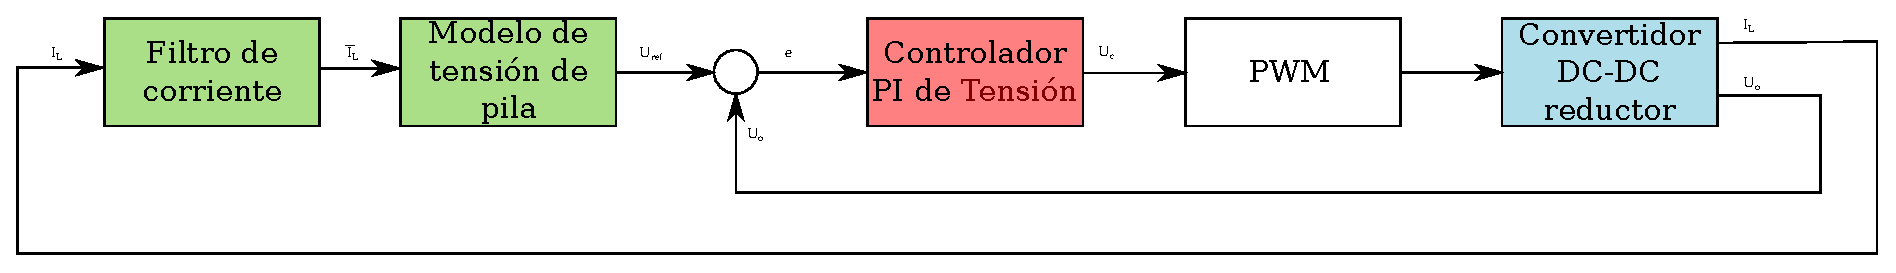
\includegraphics[width=11cm]{gfx/esquema_control.eps}
  \caption{Esquema general de control}
  \label{fig:esquema_control}
\end{figure}

\subsection{Filtro de corriente}
Conforme a la estructura presentada en la fig. \ref{fig:esquema_control} y guardando cierta analogía con del diseño el modelo de control utilizado para el
elevador (fig. \ref{fig:modelo_elevador}), nuevamente se hace necesario el uso de un filtro de corriente que rechace las componentes de frecuencia generadas
por el PWM.

Para el modelo del emulador, sin embargo, la utilización del filtro de corriente cumple una función adicional además del rechazo del rizado producido por
la operación natural del sistema de potencia. En la sec. \ref{sub:sintonia_elevador} se mencionó la necesidad de diferenciar los comportamientos dinámicos
de los diferentes lazos de realimentación con el fin de que las aproximaciones utilizadas para adaptar el esquema de control basado en controladores lineales
sea efectiva. Para aquel caso, fue necesario que la inclusión de los controladores PI permitiera corregir el error de seguimiento a la referencia y distinguir
la velocidad en que ambos lazos operaban, considerando que el lazo de corriente es más rápido. Para el modelo del emulador se ha intercambiado el orden de los
lazos de control. Esto implica una complicación ya que hay que modificar la dinámica del lazo de corriente de modo que sea haga más lento que el de tensión.

Por lo tanto el filtro que se agrega al sistema de control debe ser capaz de filtrar el rizado y reducir el ancho de banda en la medida que la dinámica resultante
provea estabilidad aceptable al sistema. No obstante, la reducción del ancho de banda de un modo muy drástico conduce a limitar la velocidad de respuesta
del convertidor. Es por ello que el diseño del filtro supuso hacer frente a una relación de compromiso entre el correcto desempeño
del emulador y la obtención de un ancho de banda suficiente para que en una etapa posterior se pueda modificar el emulador incluyendo también el comportamiento dinámico
del sistema de celdas de combustible completo. Para ello es necesario identificar el orden de las constantes de tiempo bajo las que éste funciona. Según los modelos 
utilizados, las constantes de tiempo más pequeñas corresponden al flujo de reactivos a través de los colectores de los electrodos y son del orden de las centenas de 
milisegundos ($100ms$), lo que significa que hay que tener al menos un ancho de banda de $10Hz$ para cumplir con este requerimiento. La eliminación de las componentes
de frecuencia introducidas por el PWM queda cumplida mediante la reducción del ancho de banda, ya que éstas se ubican alrededor de los $20kHz$. La dinámica del lazo
interno se encuentra por encima de los $700Hz$ y por esto se decidió que un filtro con una frecuencia de $100Hz$ sería apropiado.

La estructuras posibles de los filtros discretos lineales se definen a partir de la longitud de la respuesta al impulso. Por un lado se tienen los filtros de respuesta
al impulso finita (FIR) y por otro los de respuesta al impulso infinita (IIR). Cada uno de ellos tienen características que los vuelven ventajosos o contraproducentes
según la aplicación. Los filtros FIR poseen muchas cualidades que los hacen atractivos a la hora de elegir un filtro; algunas de ellas son que poseen fase lineal y son
inherentemente estables aunque normalmente requieren mayor cantidad de recursos computacionales para ser ejecutados. Por otro lado los filtros IIR pueden verse como
la contraparte discreta de los filtros analógicos, y sus especificaciones pueden provenir de ellos, aunque debe comprobarse su estabilidad y no debe resultar de importancia
la distorsión de fase que introducen, a diferencia de los FIR, cuya distorsión puede eliminarse por completo. Para la realización de cada una de estas estructuras
se aplican diferentes técnicas, aunque para cada problema en particular se utiliza una estructura diferente. Si lo que se desea es obtener un filtro de con bandas de
transición estrechas y de mayor eficiencia computacional se prefieren los filstros IIR. Si los requerimientos son relajados respecto a los intervalos de las bandas de transición
y la eficiencia computacional no es de importancia, se eligen los filtros FIR.

Para poder realizar el filtrado de las componentes de mayor frecuencia, correspondientes al PWM, hubo que realizar un muestreo rápido cuya tasa fuera mayor a $40kHz$
para cumplir con las condiciones del teorema de muestreo. Es por ello que los sensores adquieren muestras a una tasa de $200kHz$ y esto trae como consecuencia que la
frecuencia de corte elegida para el diseño del filtro resulta muy chica respecto a ella. Esto deriva en que la estructura de la realización debe ser IIR, ya que en
contraste, los filtros FIR se vuelven más complejos mientras el intervalo que separa la frecuencia de corte y la de muestreo es más alta.

\begin{figure}[H]
 \centering
 \subfloat[Filtro bicuadrático en forma directa I]{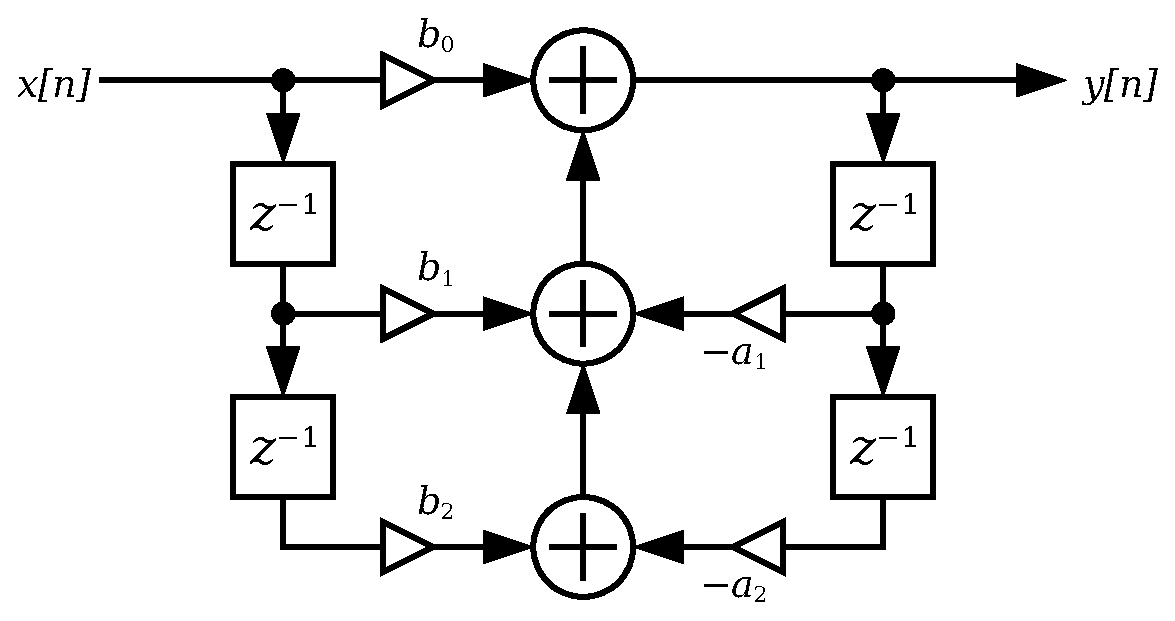
\includegraphics[width=5cm]{gfx/forma_directa_I.eps}\label{fig:forma_directa_I}} \quad
 \subfloat[Filtro bicuadrático en forma directa II]{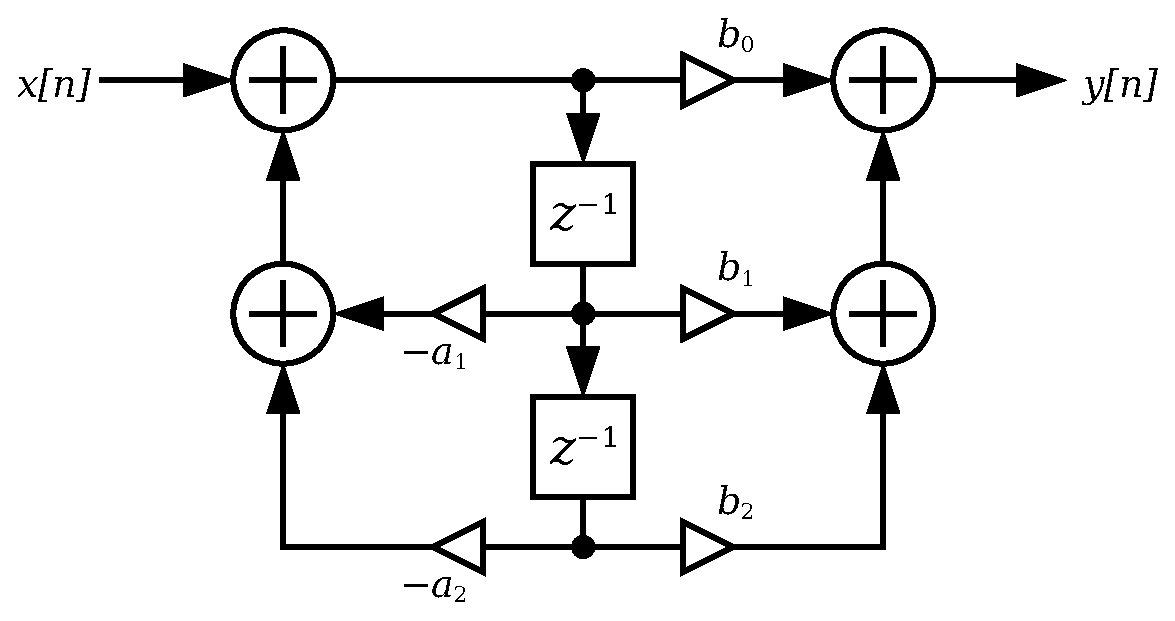
\includegraphics[width=5cm]{gfx/forma_directa_II.eps}\label{fig:forma_directa_II}}
 \caption{Formas directas de filtros IIR}
 \label{fig:forma_directa}
\end{figure}

La implementación de los filtros IIR se puede efectuar siguiendo alguna de varias estructuras. Las más comunes son las formas directas, cascada y paralelo. Dentro
de las formas directas hay dos posibilidades: las de tipo I y II (figuras \ref{fig:forma_directa_I} y \ref{fig:forma_directa_II}). 
La exigencia en la especificación de las bandas de transición hacen que la respuesta pueda cambiar en gran medida debido a los errores de cuantización.
Por eso, para el trabajo se utilizó una estructura conocida como cascada de \emph{secciones de segundo orden} ya que permite disminuir la sensibilidad del error de
cuantización debido a la longitud finita de las palabras de memoria. En la fig. \ref{fig:respuesta_filtro_corriente} se muestra la respuesta en frecuencia del filtro 
implementado. Corresponde a un filtro de tercer orden, cuya matriz de coeficientes se muestra a continuación:

\begin{tabular}{|c|c|c|c|c|c|c|}
 \hline
		&	$b_0$	&	$b_1$	&	$b_2$	&	$a_0=1$	&	$a_1$	&	$a_2$	\\ \hline
Primera sección	&	1	&	-2	&	1	&	1	&	-1,9965	&	0,9965	\\
Segunda sección	&	2	&	2	&	0	&	1	&	-0,9947	&	0	\\ \hline
\end{tabular}

Los coeficientes presentados le confieren al filtro sus características en frecuencia, sin embargo es necesario aclarar se han utilizado ganancias
para escalar los valores entre secciones y así evitar el desbordamiento del límite de palabra.

\begin{figure}[H]
 \centering
 \subfloat[Respuesta en frecuencia del filtro implementado]{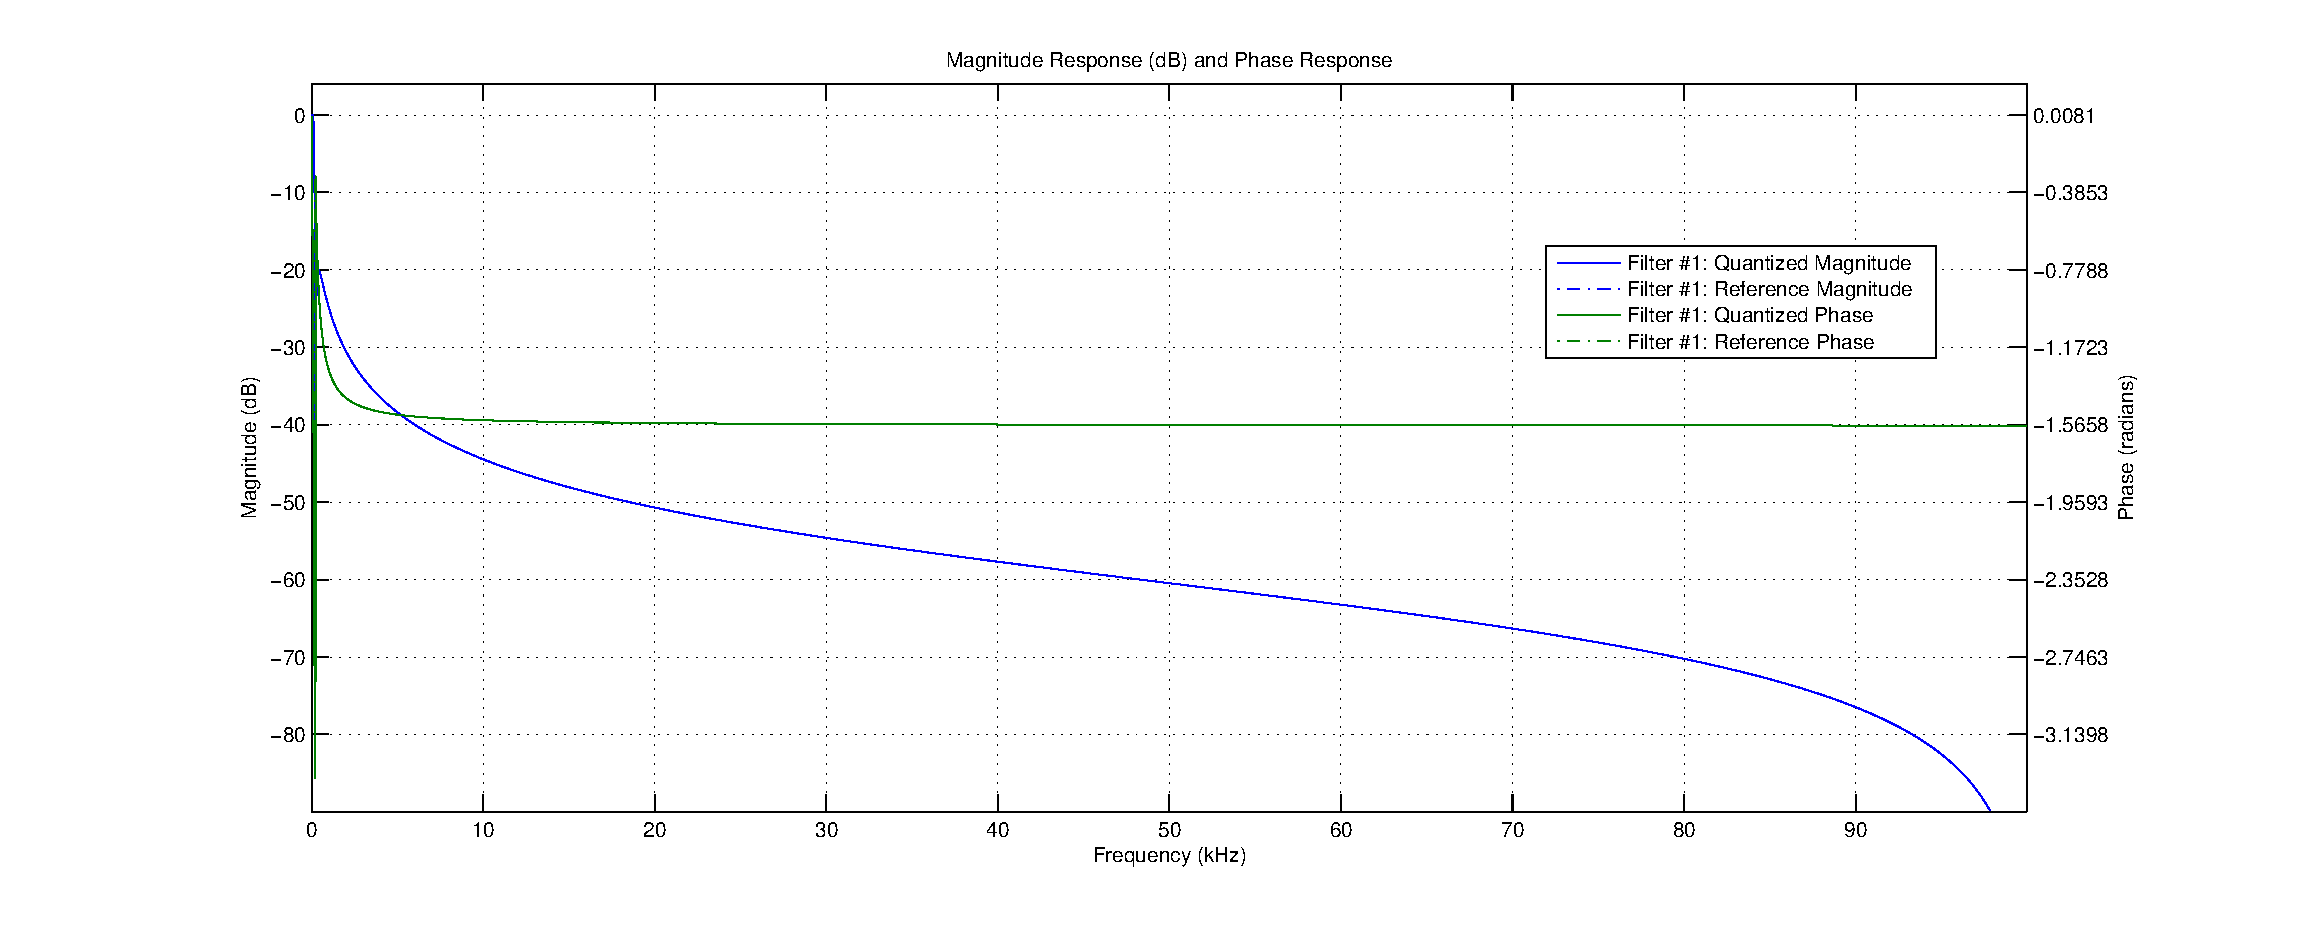
\includegraphics[width=10cm]{gfx/respuesta_filtro.eps}\label{fig:respuesta_filtro}} \\
 \subfloat[Ampliación de la zona del filtro correspondiente a la banda de paso]{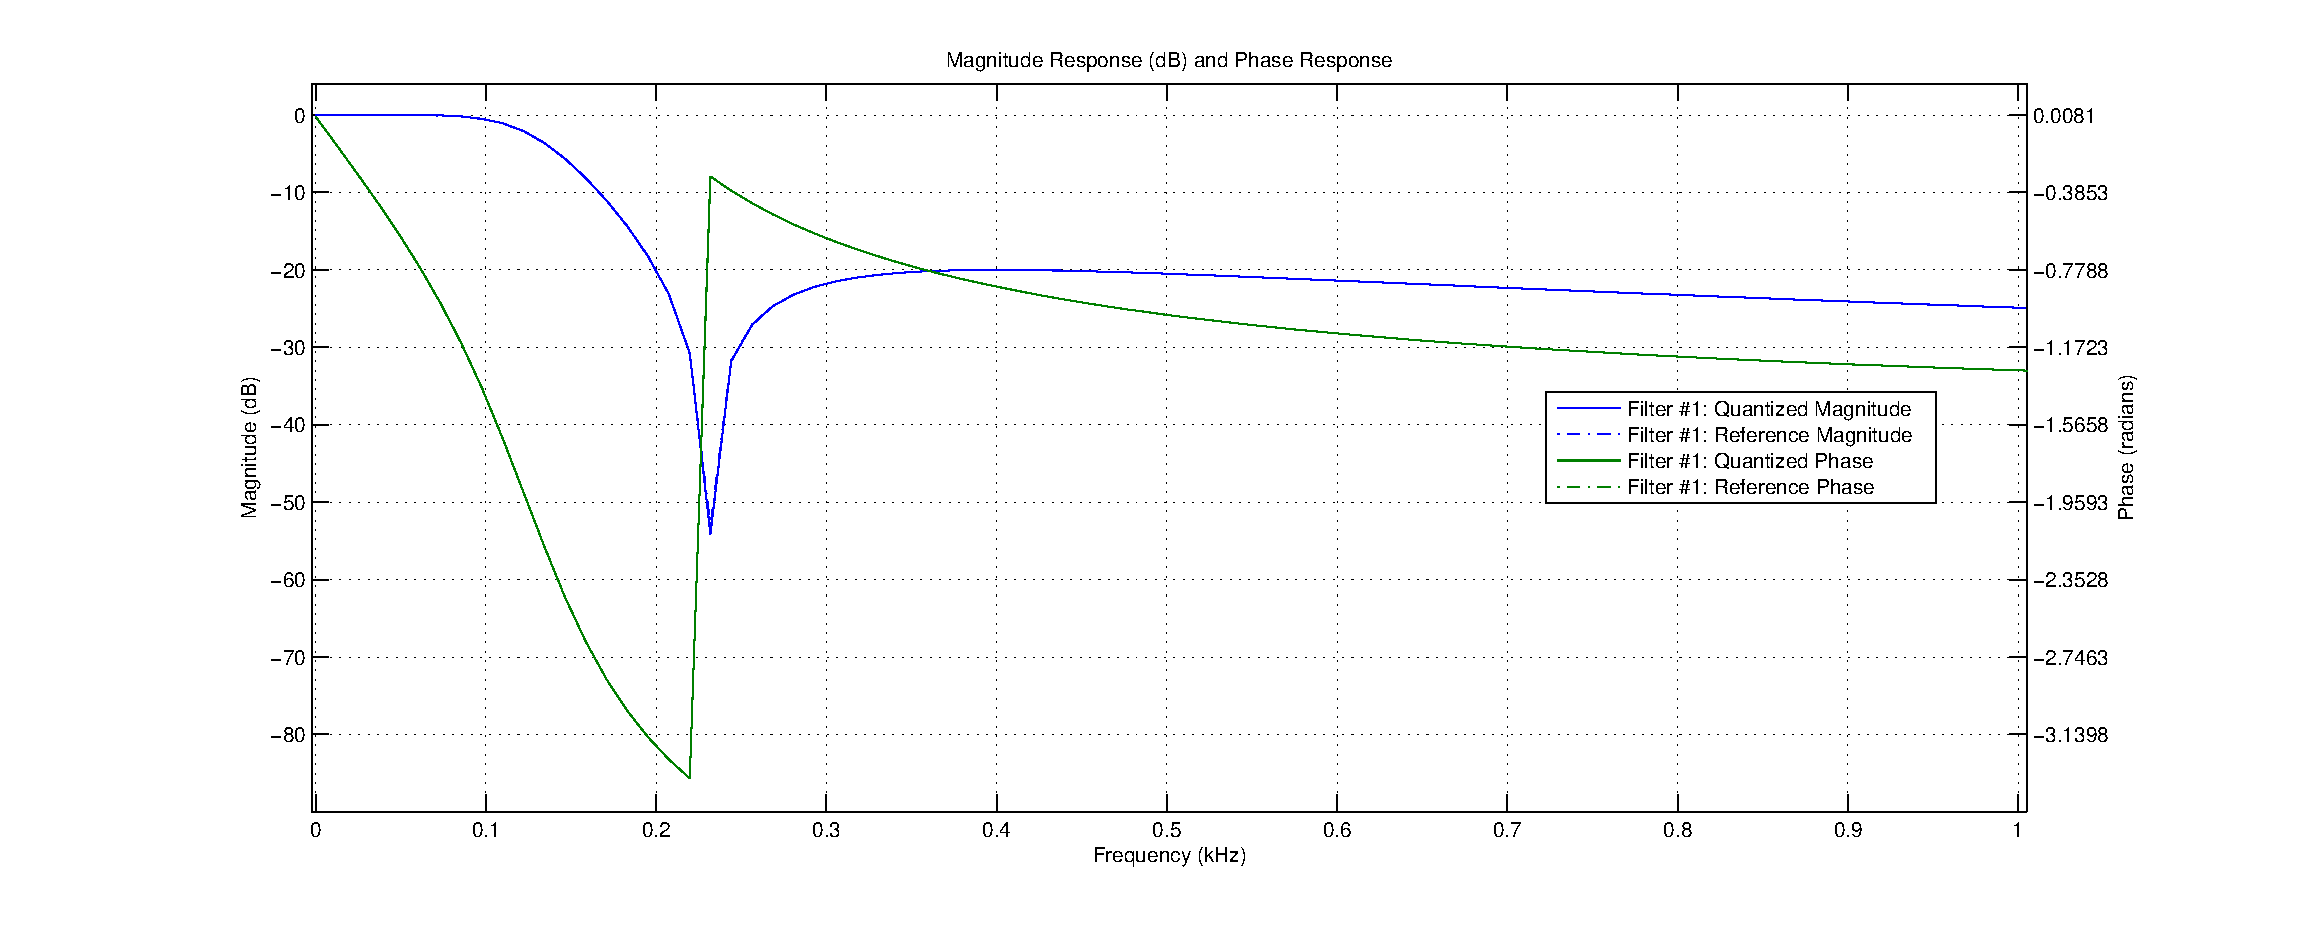
\includegraphics[width=10cm]{gfx/respuesta_filtro_ampliado.eps}\label{fig:respuesta_filtro_ampliado}}
 \caption{Respuesta en frecuencia de filtro de corriente}
 \label{fig:respuesta_filtro_corriente}
\end{figure}

\section{Simulaciones}
En esta sección se presentan los modelos realizados en Simulink de los emuladores completos y los resultados obtenidos utilizando una
carga que representa un banco de resistencias disponible en el laboratorio que se ensayó el emulador. Se adjunta a su vez el relevamiento de los puntos de polarización 
que devuelve el emulador cuya tendencia se pretende hacer coincidir con el ensayo de laboratorio.

\subsection{Modelo Fijo}
En esta sección se presentan los resultados del simulación del emulador usando el modelo fijo de tensión de pila presentado en la sec. \ref{sub:modelo_fijo}. 
En la fig. \ref{fig:modelo_emulador_1} se presenta el modelo de simulación que se usó para evaluar la funcionalidad bajo \emph{software}.
Las respuestas se encuentran en las figuras \ref{fig:respuesta_emulador_1} y \ref{fig:I-V_modelo_1} donde se puede ver el comportamiento dinámico y los puntos
de polarización, respectivamente. Tal como se previó, la respuesta dinámica es suficientemente rápida como para poder acoplar en un futuro la dinámica correspondiente
al modelo de pila completo. Por otro lado se observa que los puntos de polarización coinciden de forma precisa con los que presenta la curva del modelo utilizado.

\begin{figure}[H]
\centering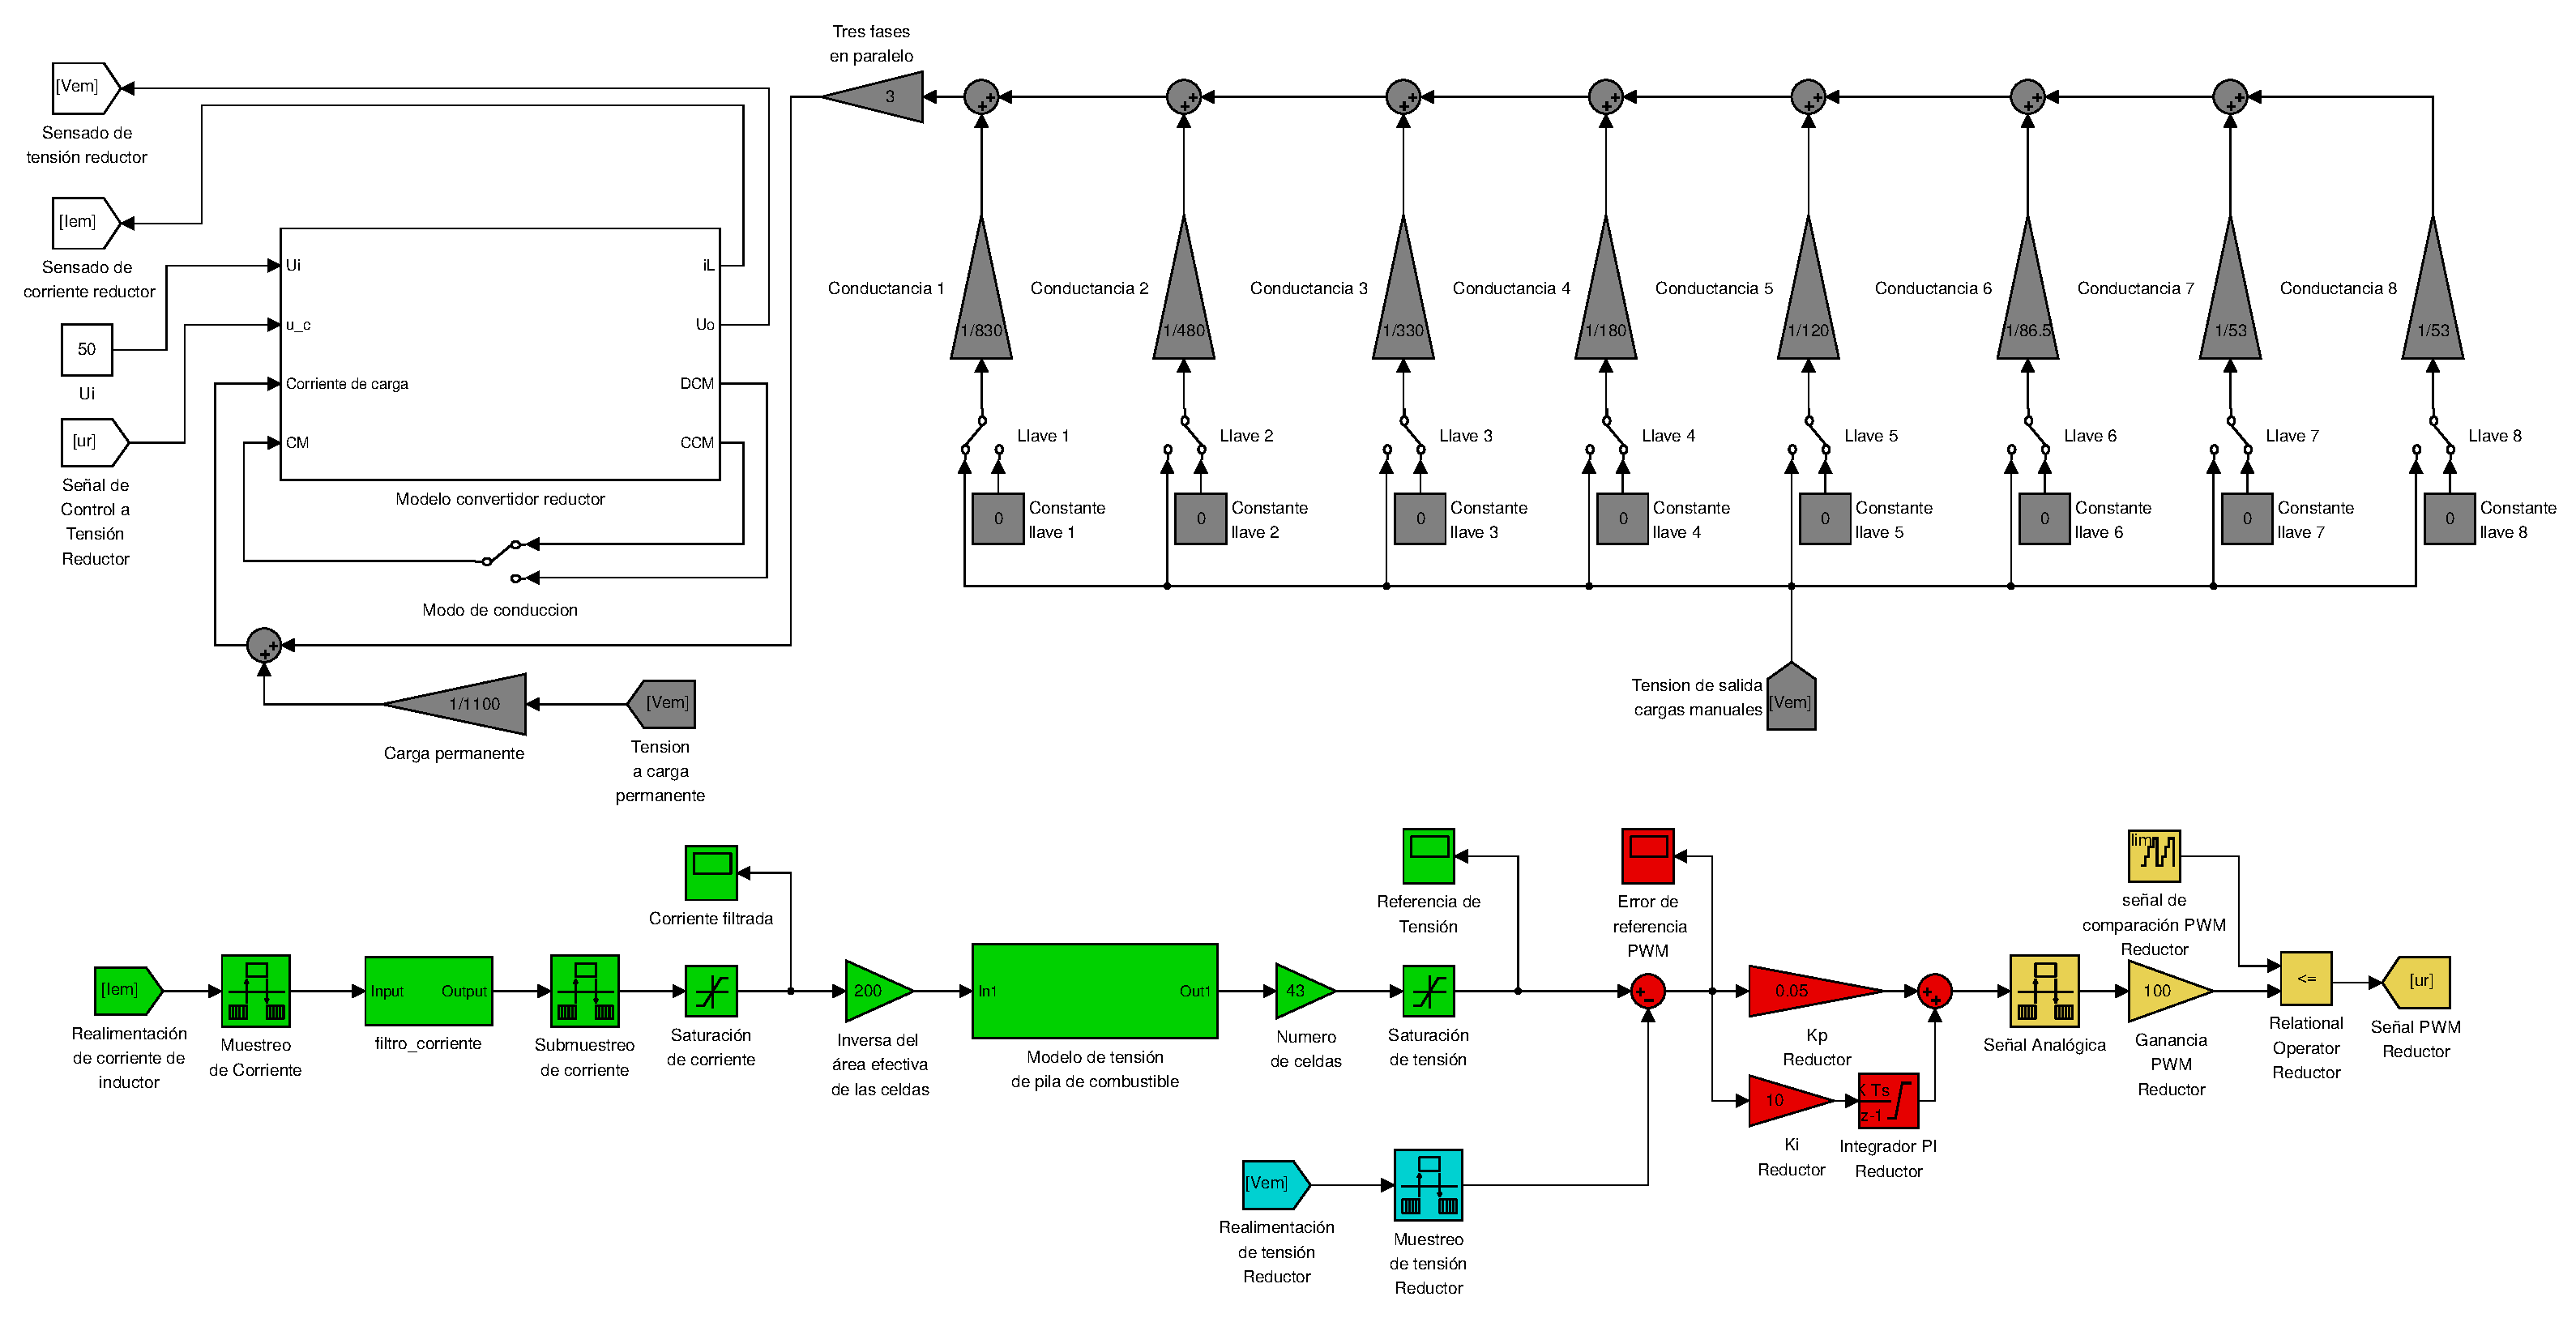
\includegraphics[width=10cm]{gfx/modelo_emulador_1.eps}
\caption{Esquema de simulink del modelo fijo}
\label{fig:modelo_emulador_1}
\end{figure}

\begin{figure}[H]
\centering
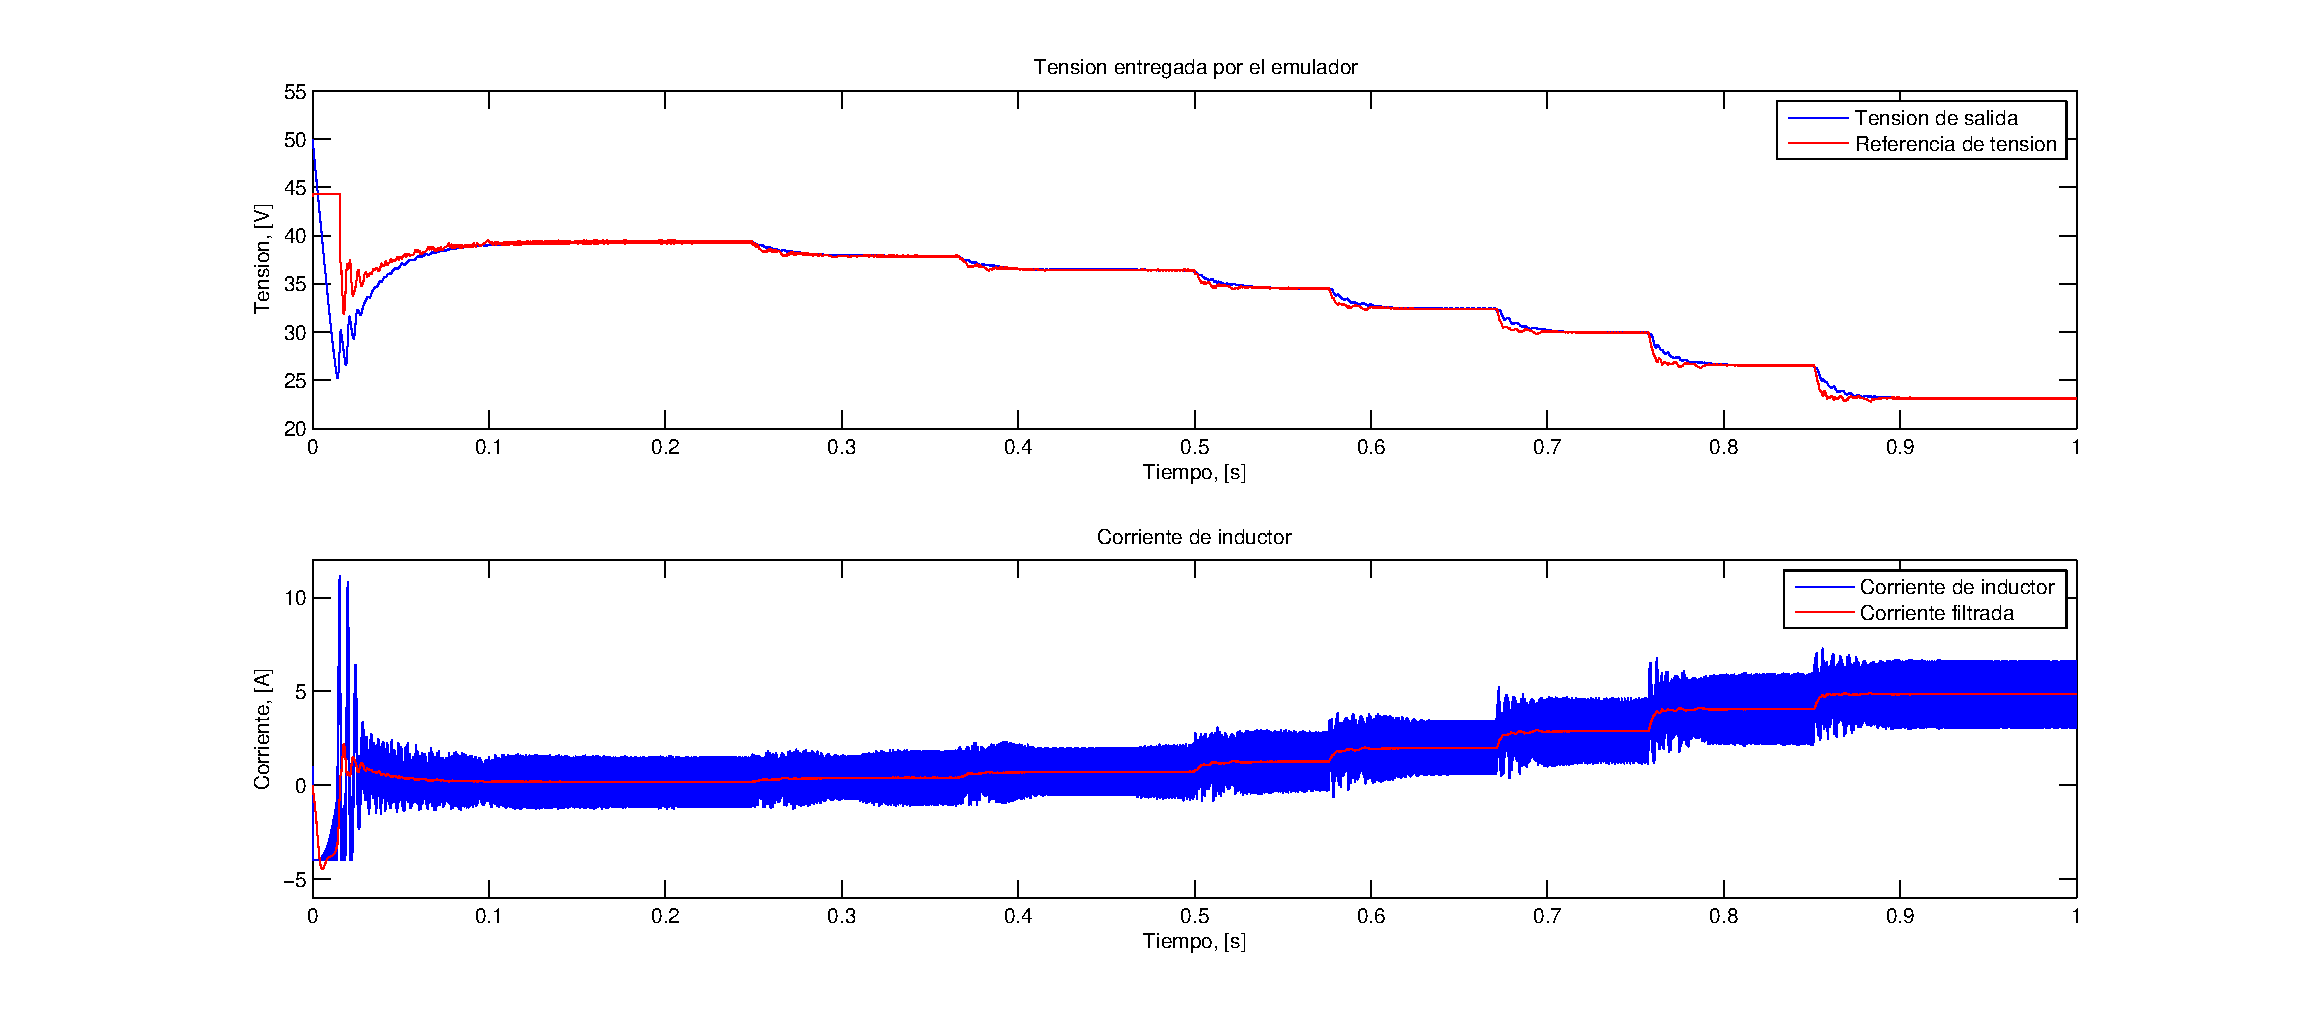
\includegraphics[width=10cm]{gfx/respuesta_emulador_1.eps}
\caption{Resultados de simulación para las magnitudes de salida del emulador}
\label{fig:respuesta_emulador_1}
\end{figure}

\begin{figure}[H]
  \centering
  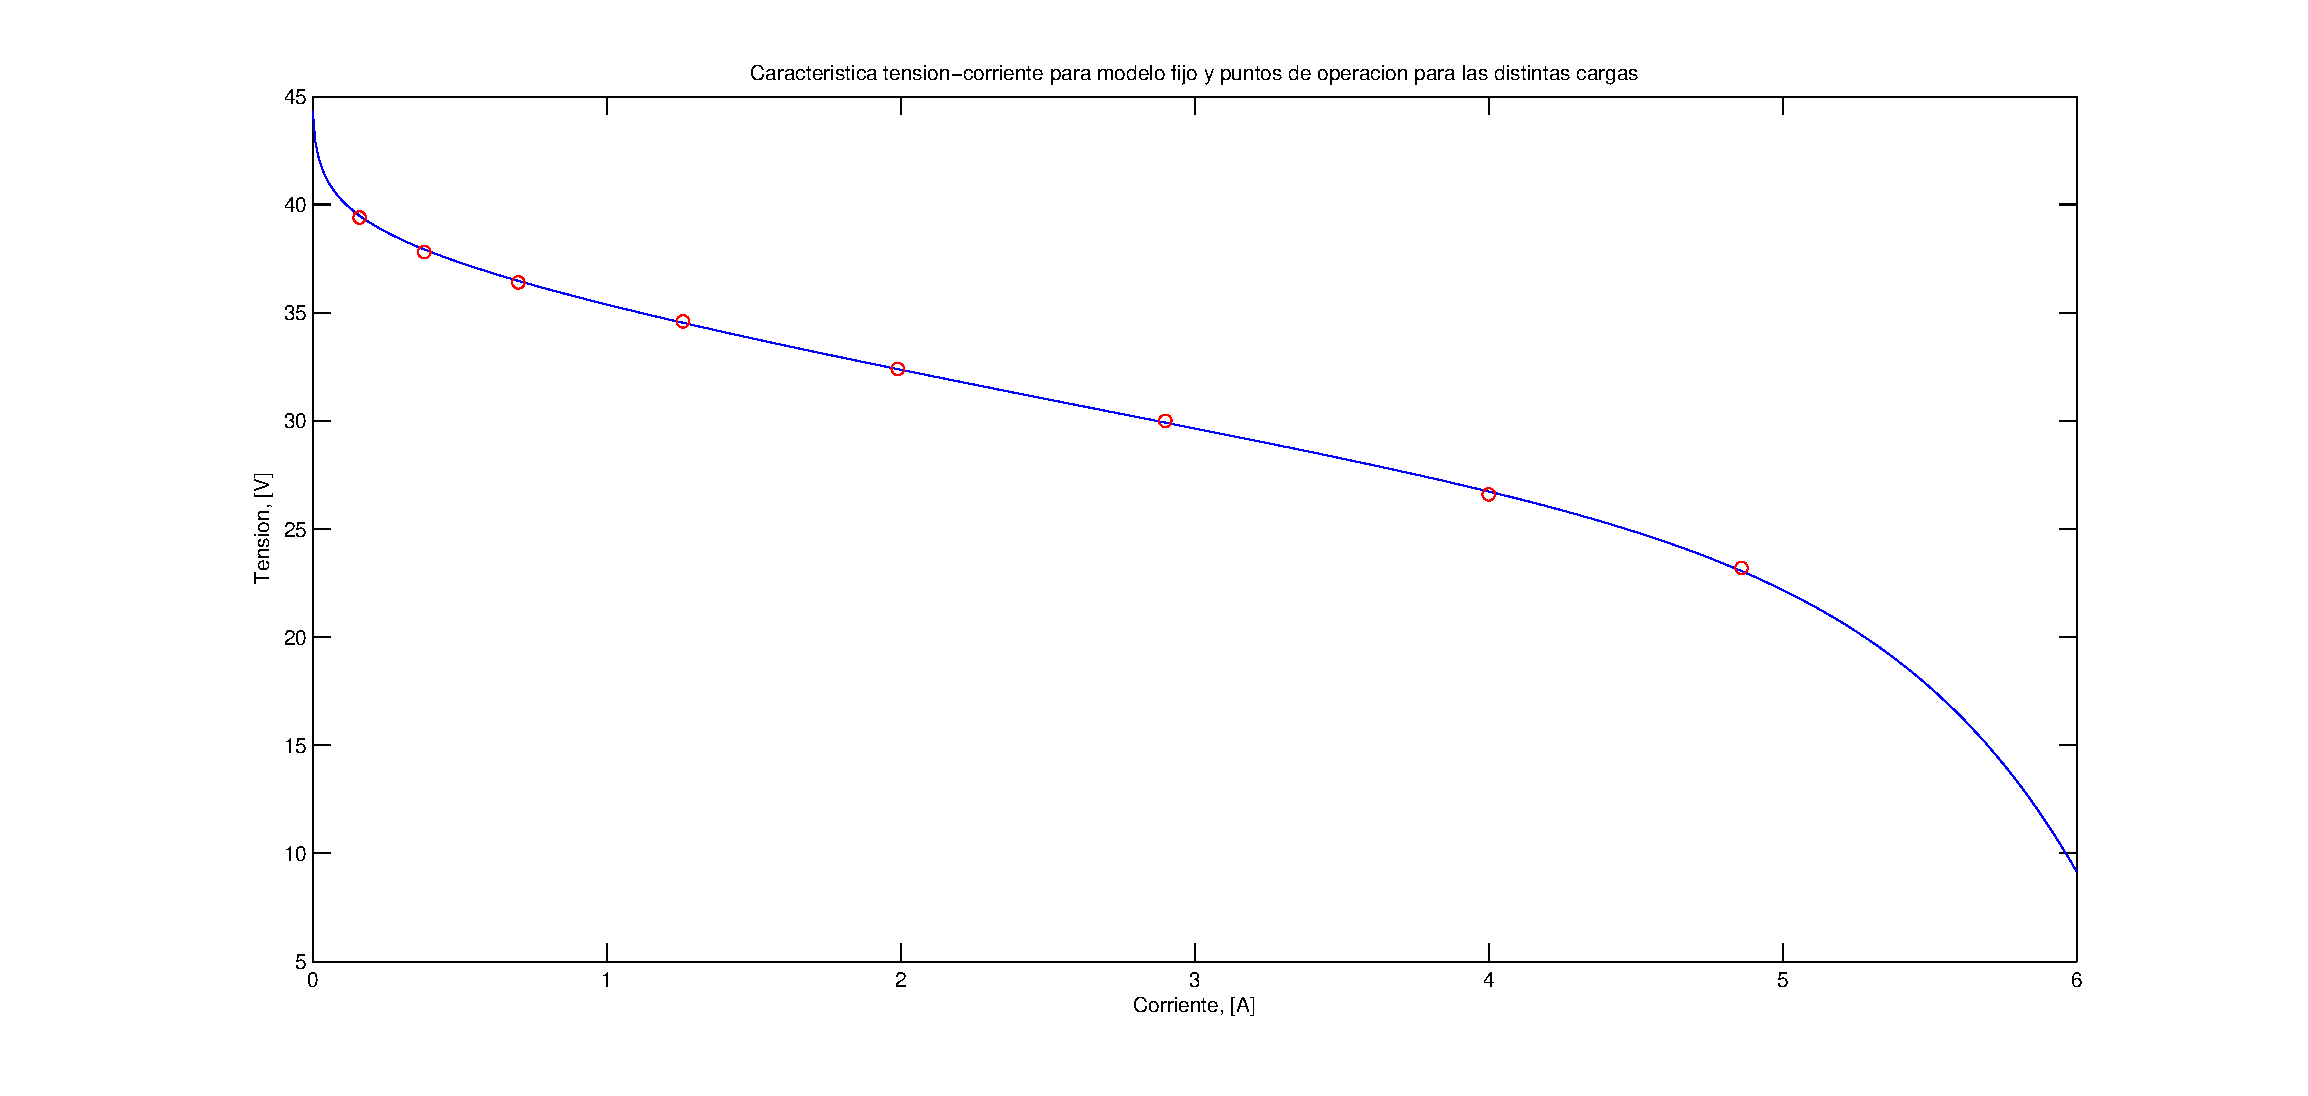
\includegraphics[width=10cm]{gfx/I-V_modelo_1.eps}
  \caption{Relevamiento de curvas para modelo fijo}
  \label{fig:I-V_modelo_1}
\end{figure}

\subsection{Modelo paramétrico}
Los resultados siguientes comprenden la simulación correspondiente al modelo que permite configurar la temperatura de las celdas de combustible y la presión
de los electrodos\footnote{se asumió que la presión de ánodo se establece igual a la de cátodo}. Los parámetros elegidos se pueden ver en el modelo de la fig.
\ref{fig:modelo_emulador_2} y corresponden a una temperatura de $70$\textcelsius y $2\,atm$ de presión en el ánodo.

\begin{figure}[H]
  \centering
  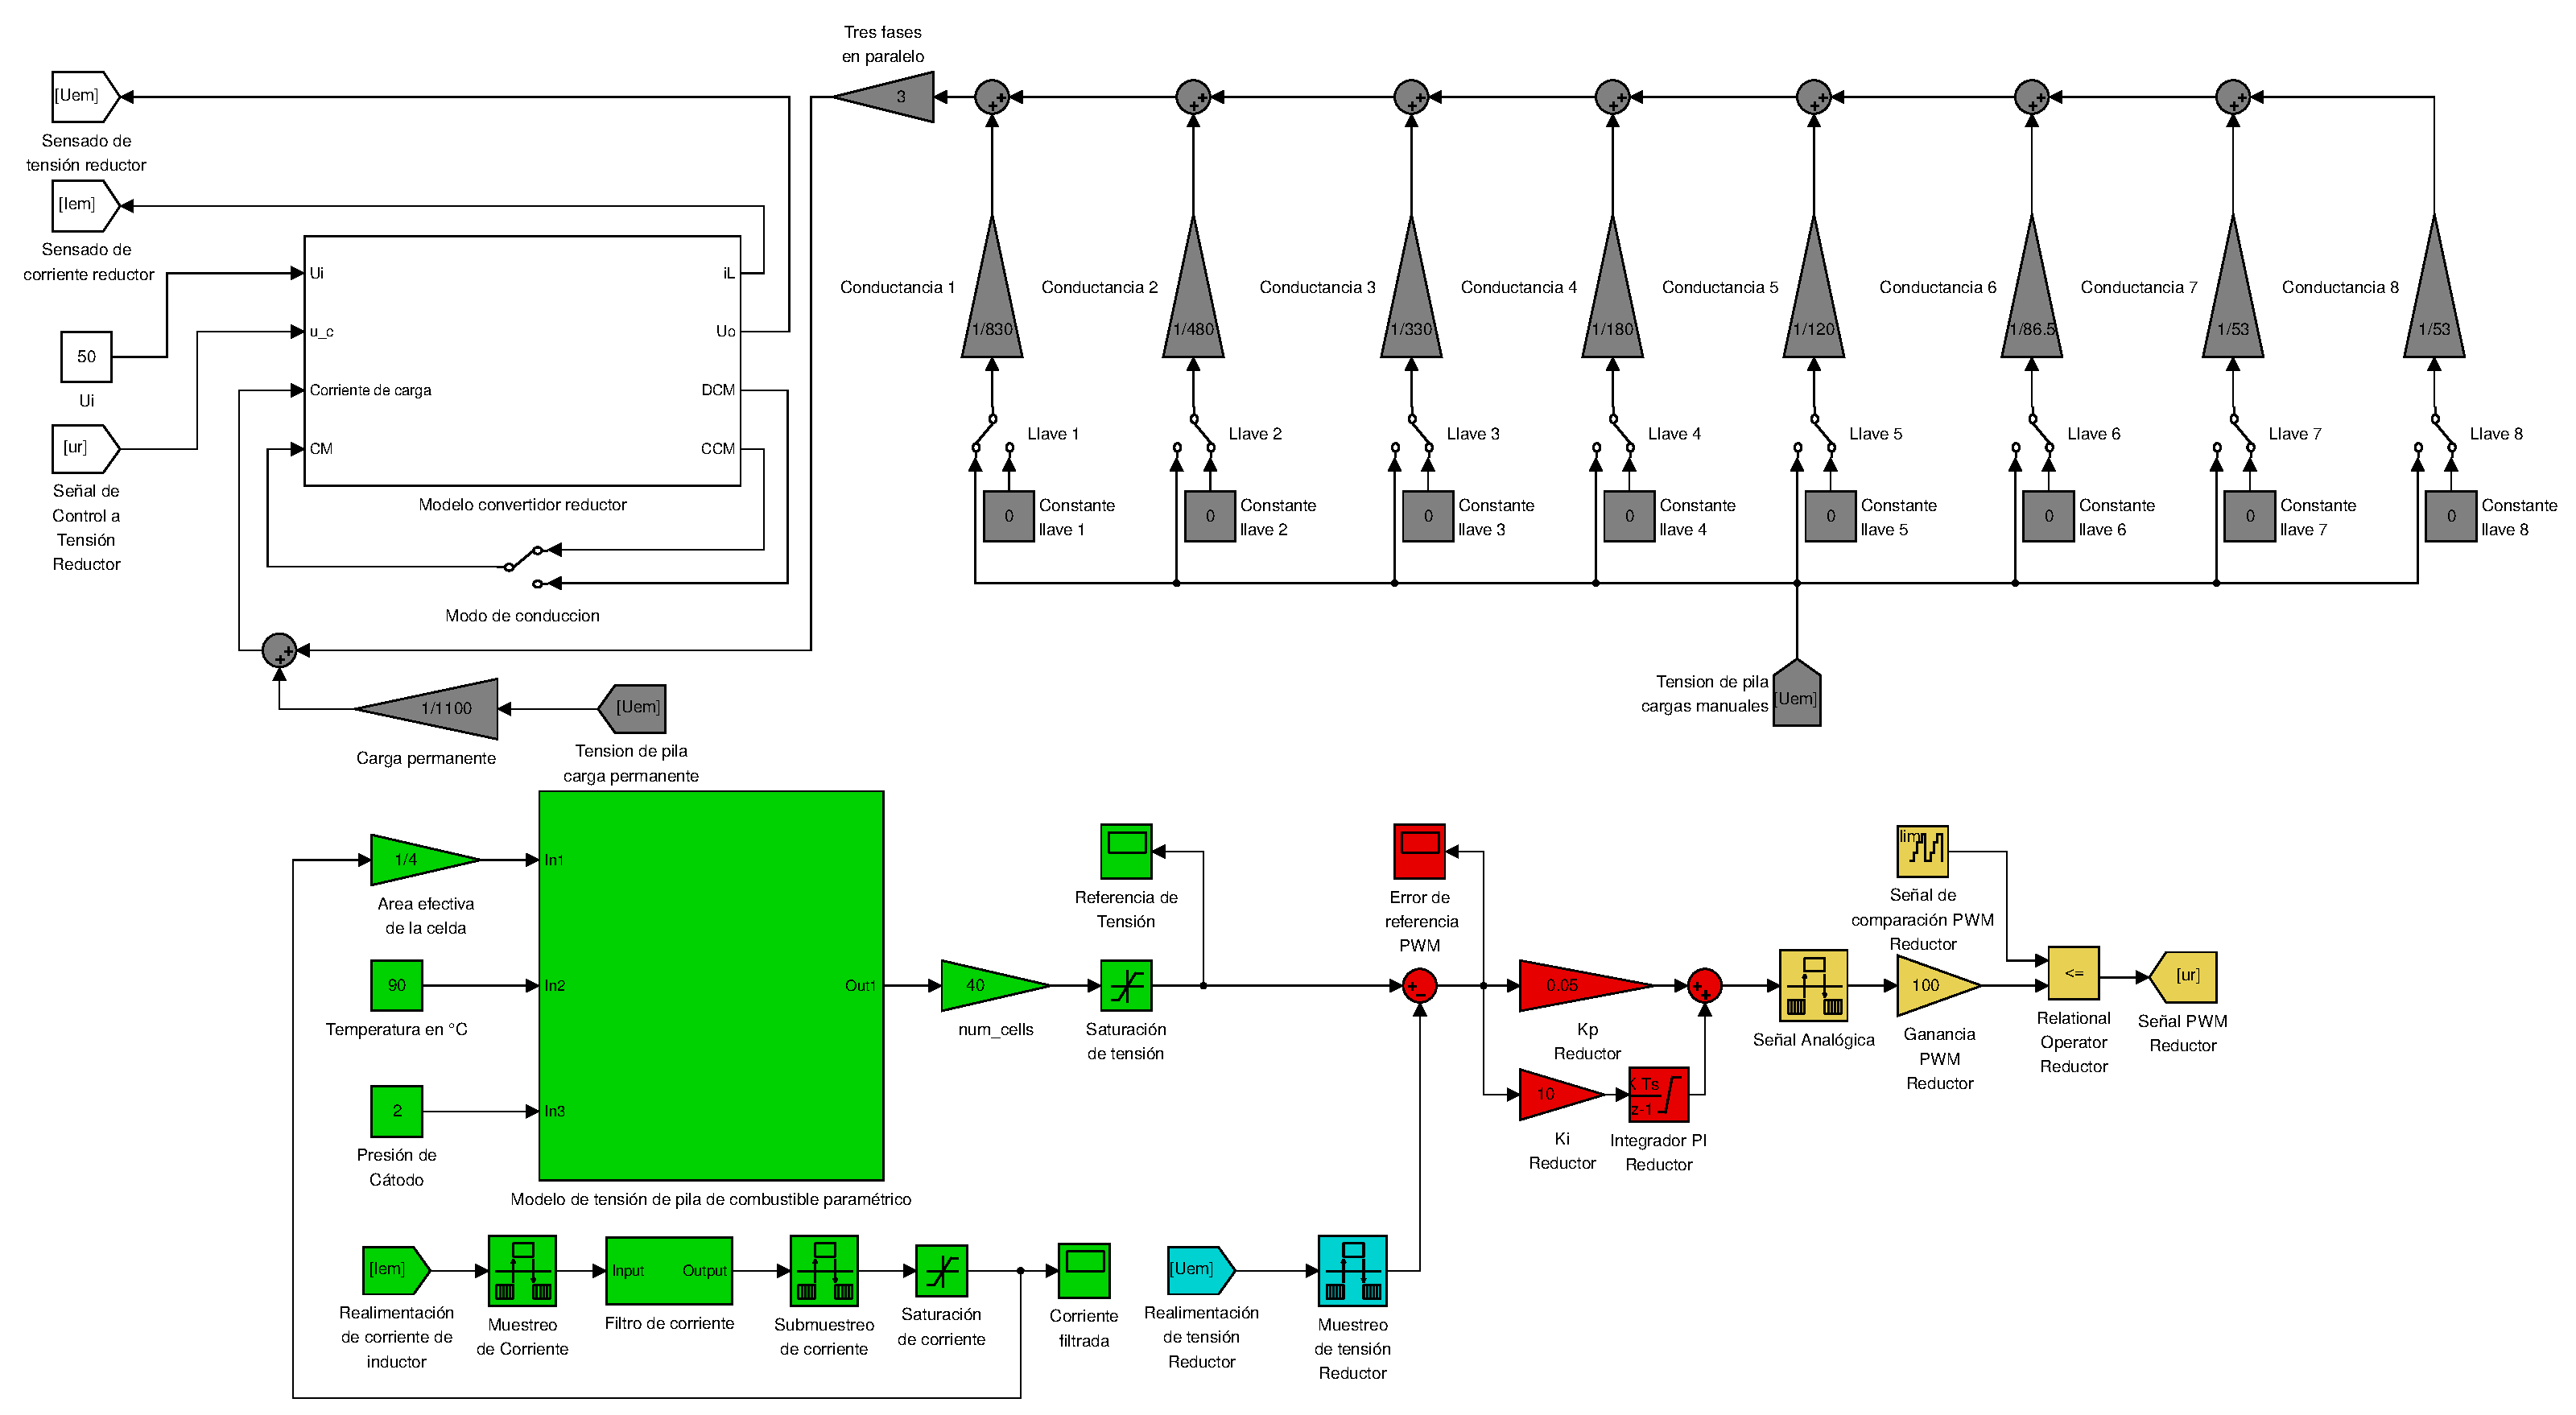
\includegraphics[width=10cm]{gfx/modelo_emulador_2.eps}
  \caption{Esquema simulink del modelo paramétrico}
  \label{fig:modelo_emulador_2}
\end{figure}

\begin{figure}[H]
  \centering
  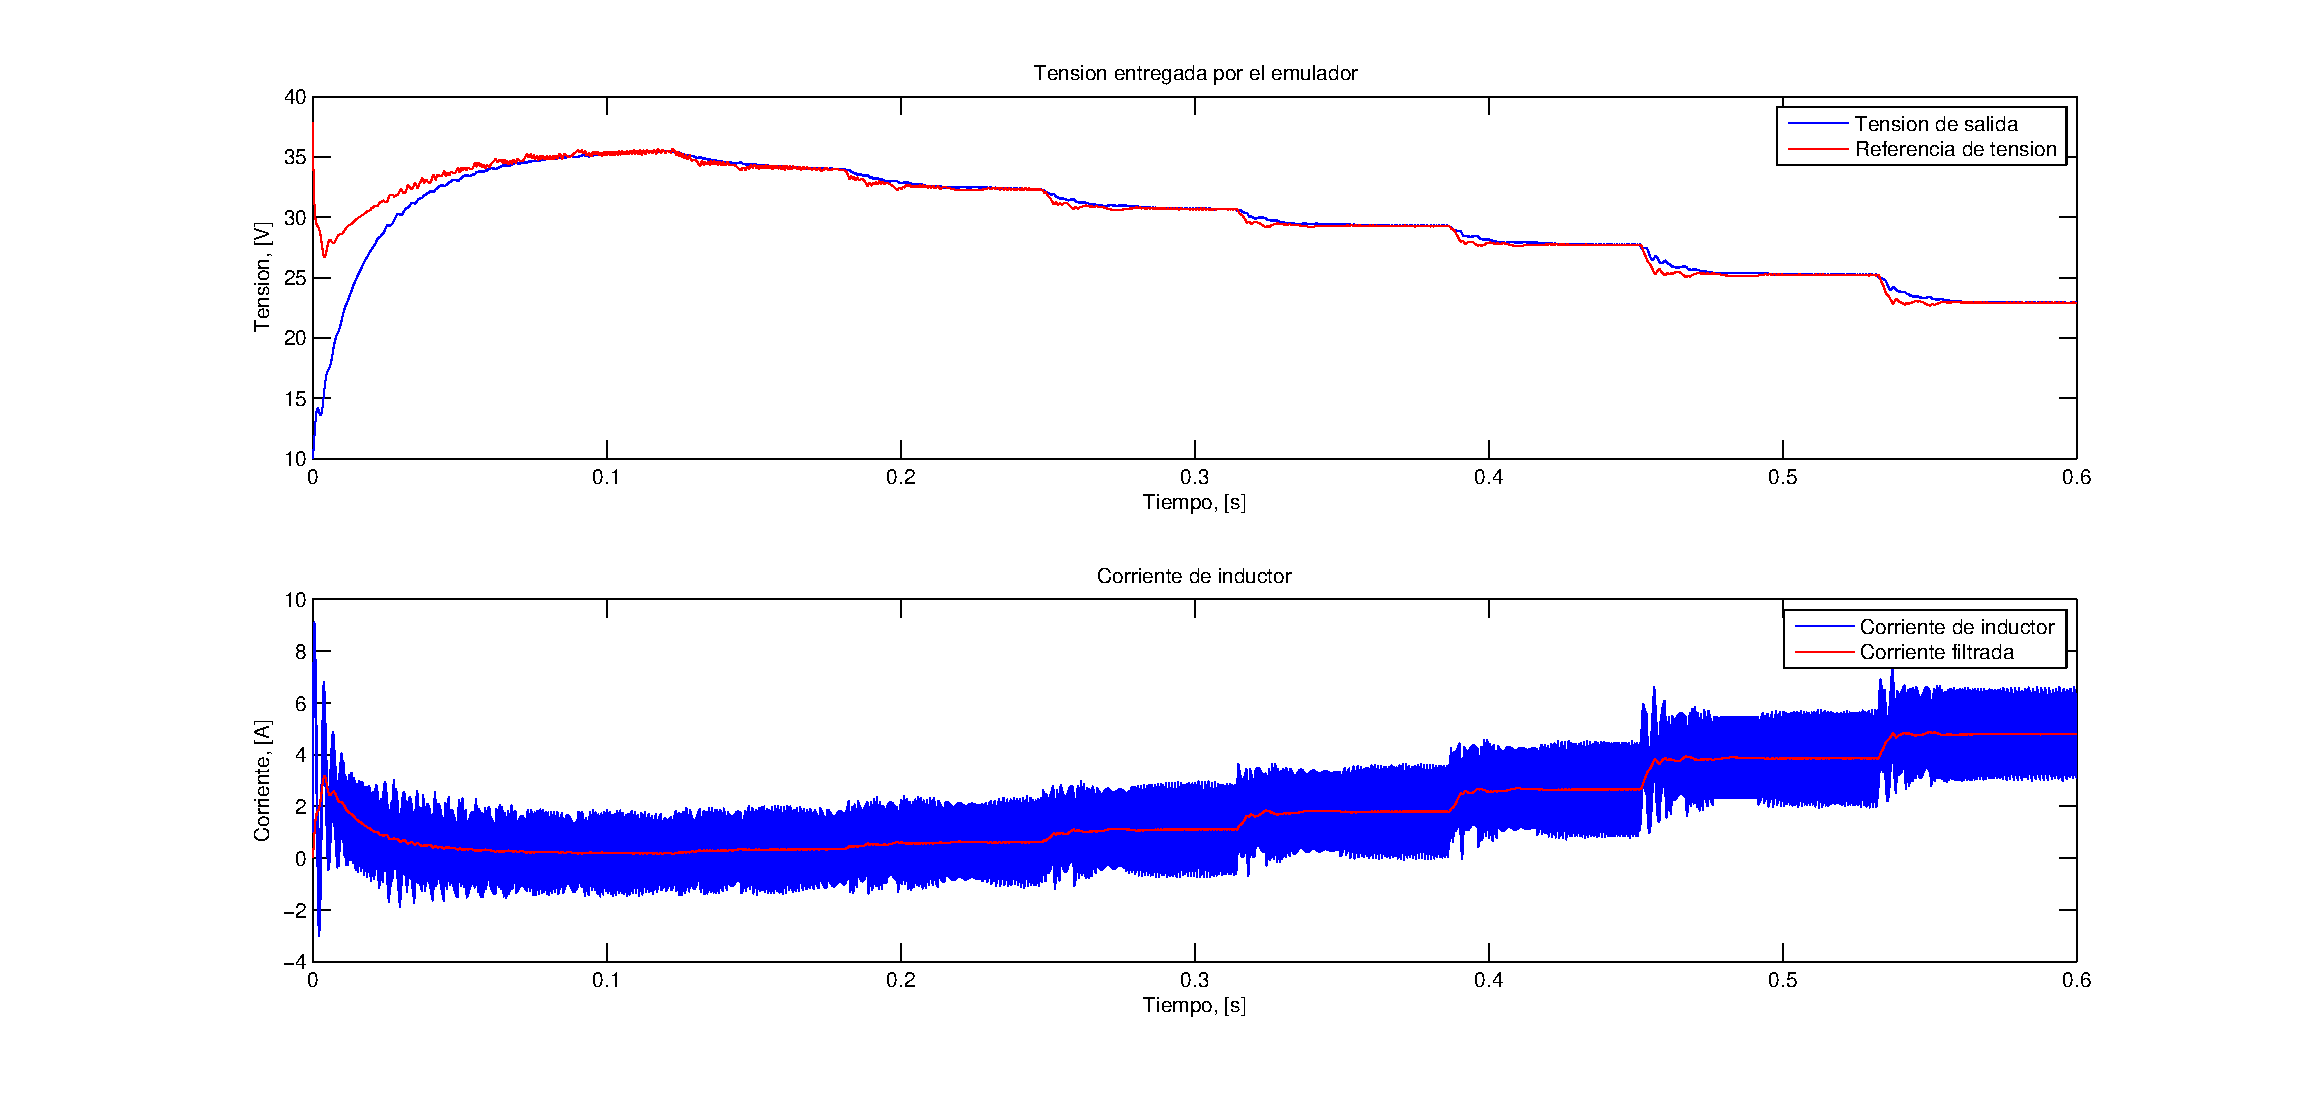
\includegraphics[width=10cm]{gfx/respuesta_emulador_2.eps}
  \caption{Resultados de simulación para las magnitudes de salida del emulador paramétrico}
\end{figure}
% 
Al igual que para el modelo anterior, los puntos de polarización ajustan con bastante precisión a la característica dada para esas condiciones
de funcionamiento.

\begin{figure}[H]
  \centering
  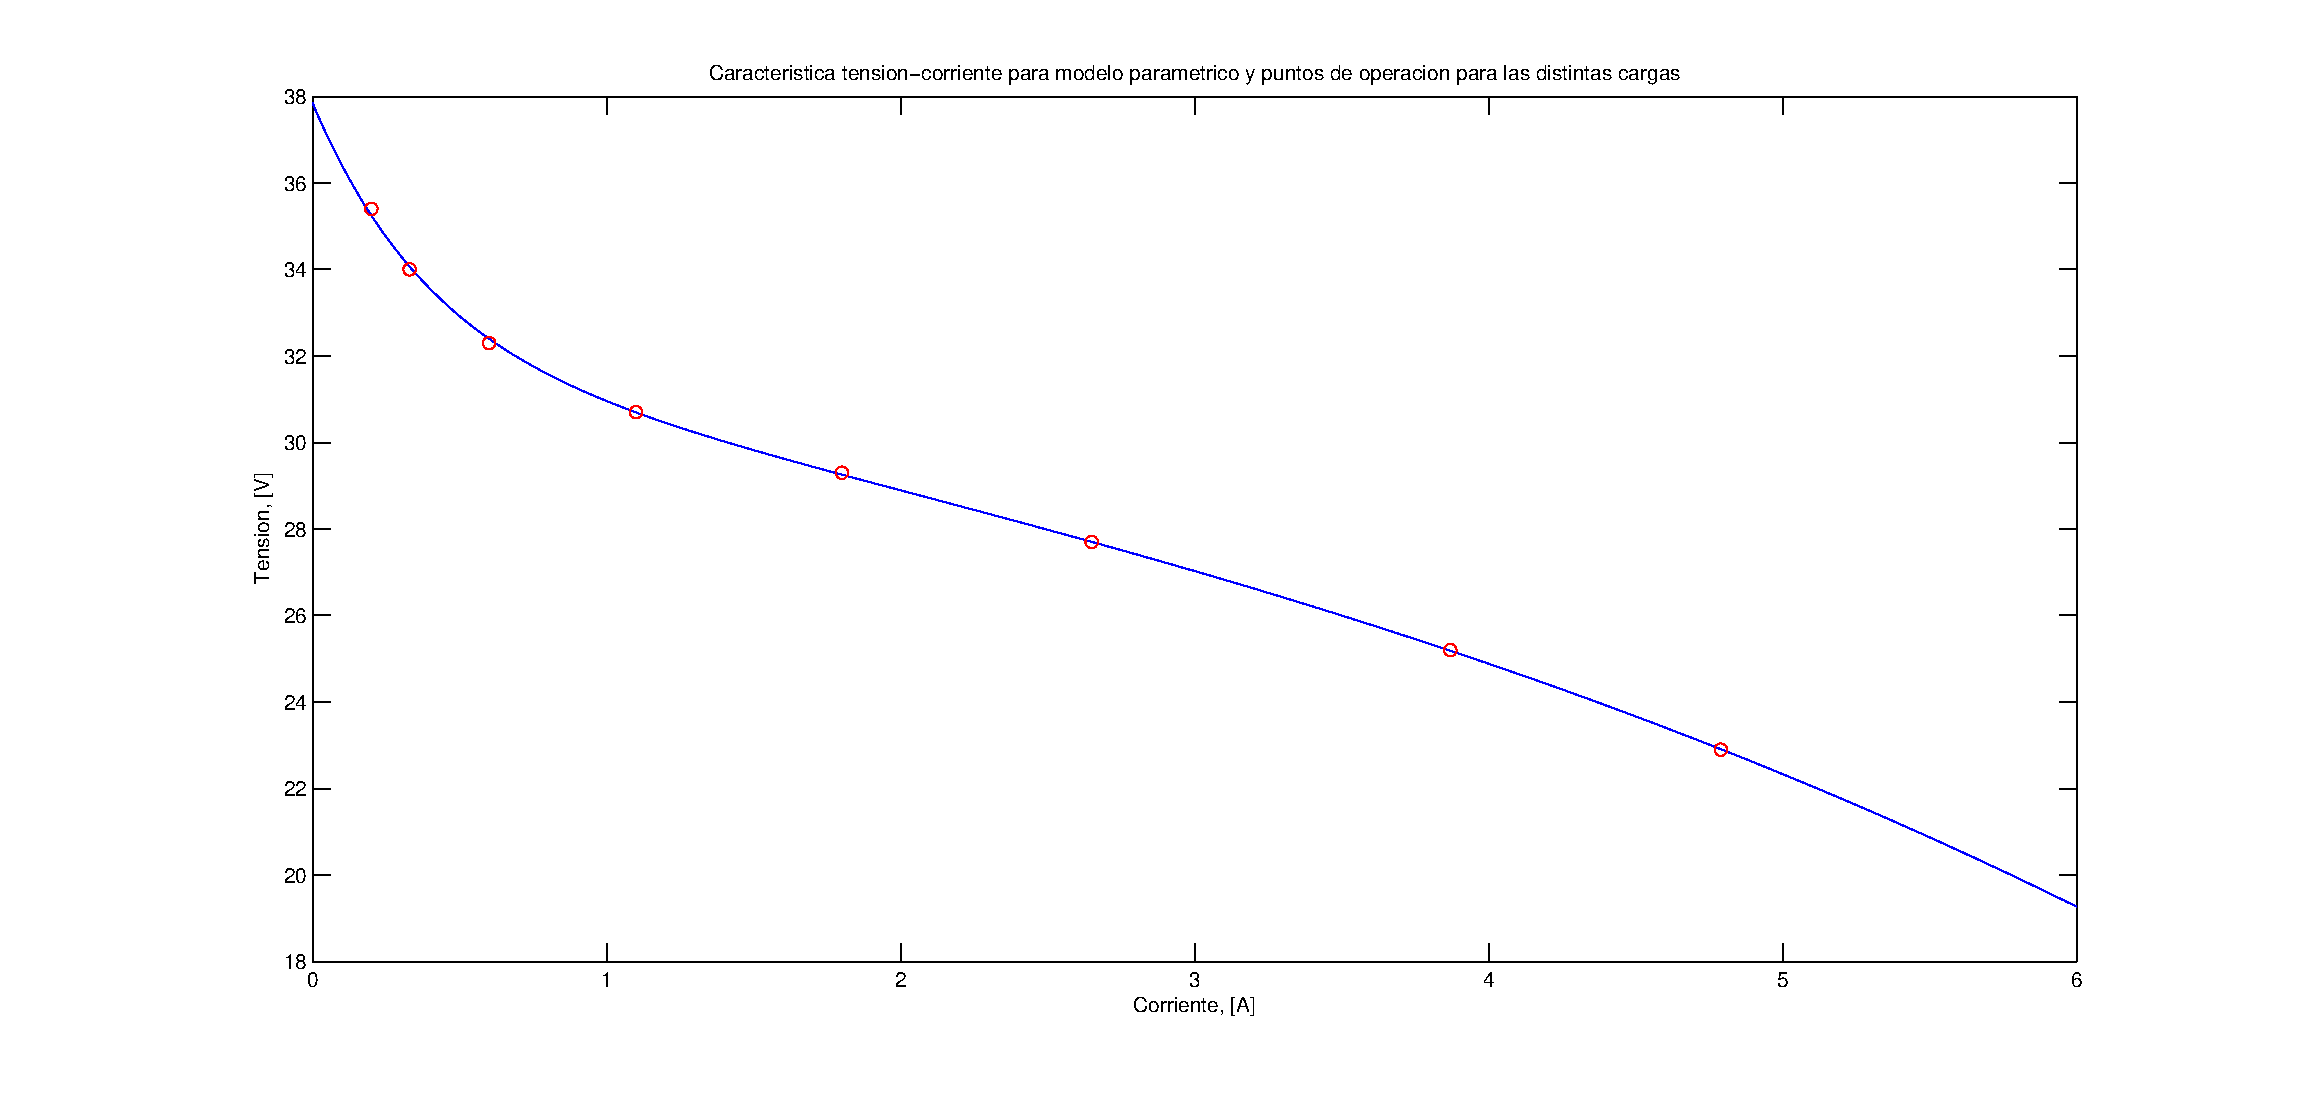
\includegraphics[width=10cm]{gfx/I-V_modelo_2.eps}
  \caption{Relevamiento de curvas para modelo paramétrico}
\end{figure}

\subsection{Operación conjunta del emulador y la etapa de potencia}
Se mostró en el cap. \ref{ch:control} que es posible en simulación, la operación conjunta de ambos módulos de potencia. En esta etapa se pretende verificar
la factibilidad del funcionamiento de la operación del emulador a diferentes cargas. Para este caso el emulador trabajó en un rango de corriente más amplio
debido a que la tensión aplicada sobre la carga es siempre 60V gracias a la acción del elevador y por ello se debió ajustar el parámetro del área efectiva
de la celda para que sea posible la operación en todo el intervalo de corriente.

\begin{figure}[H]
 \centering
 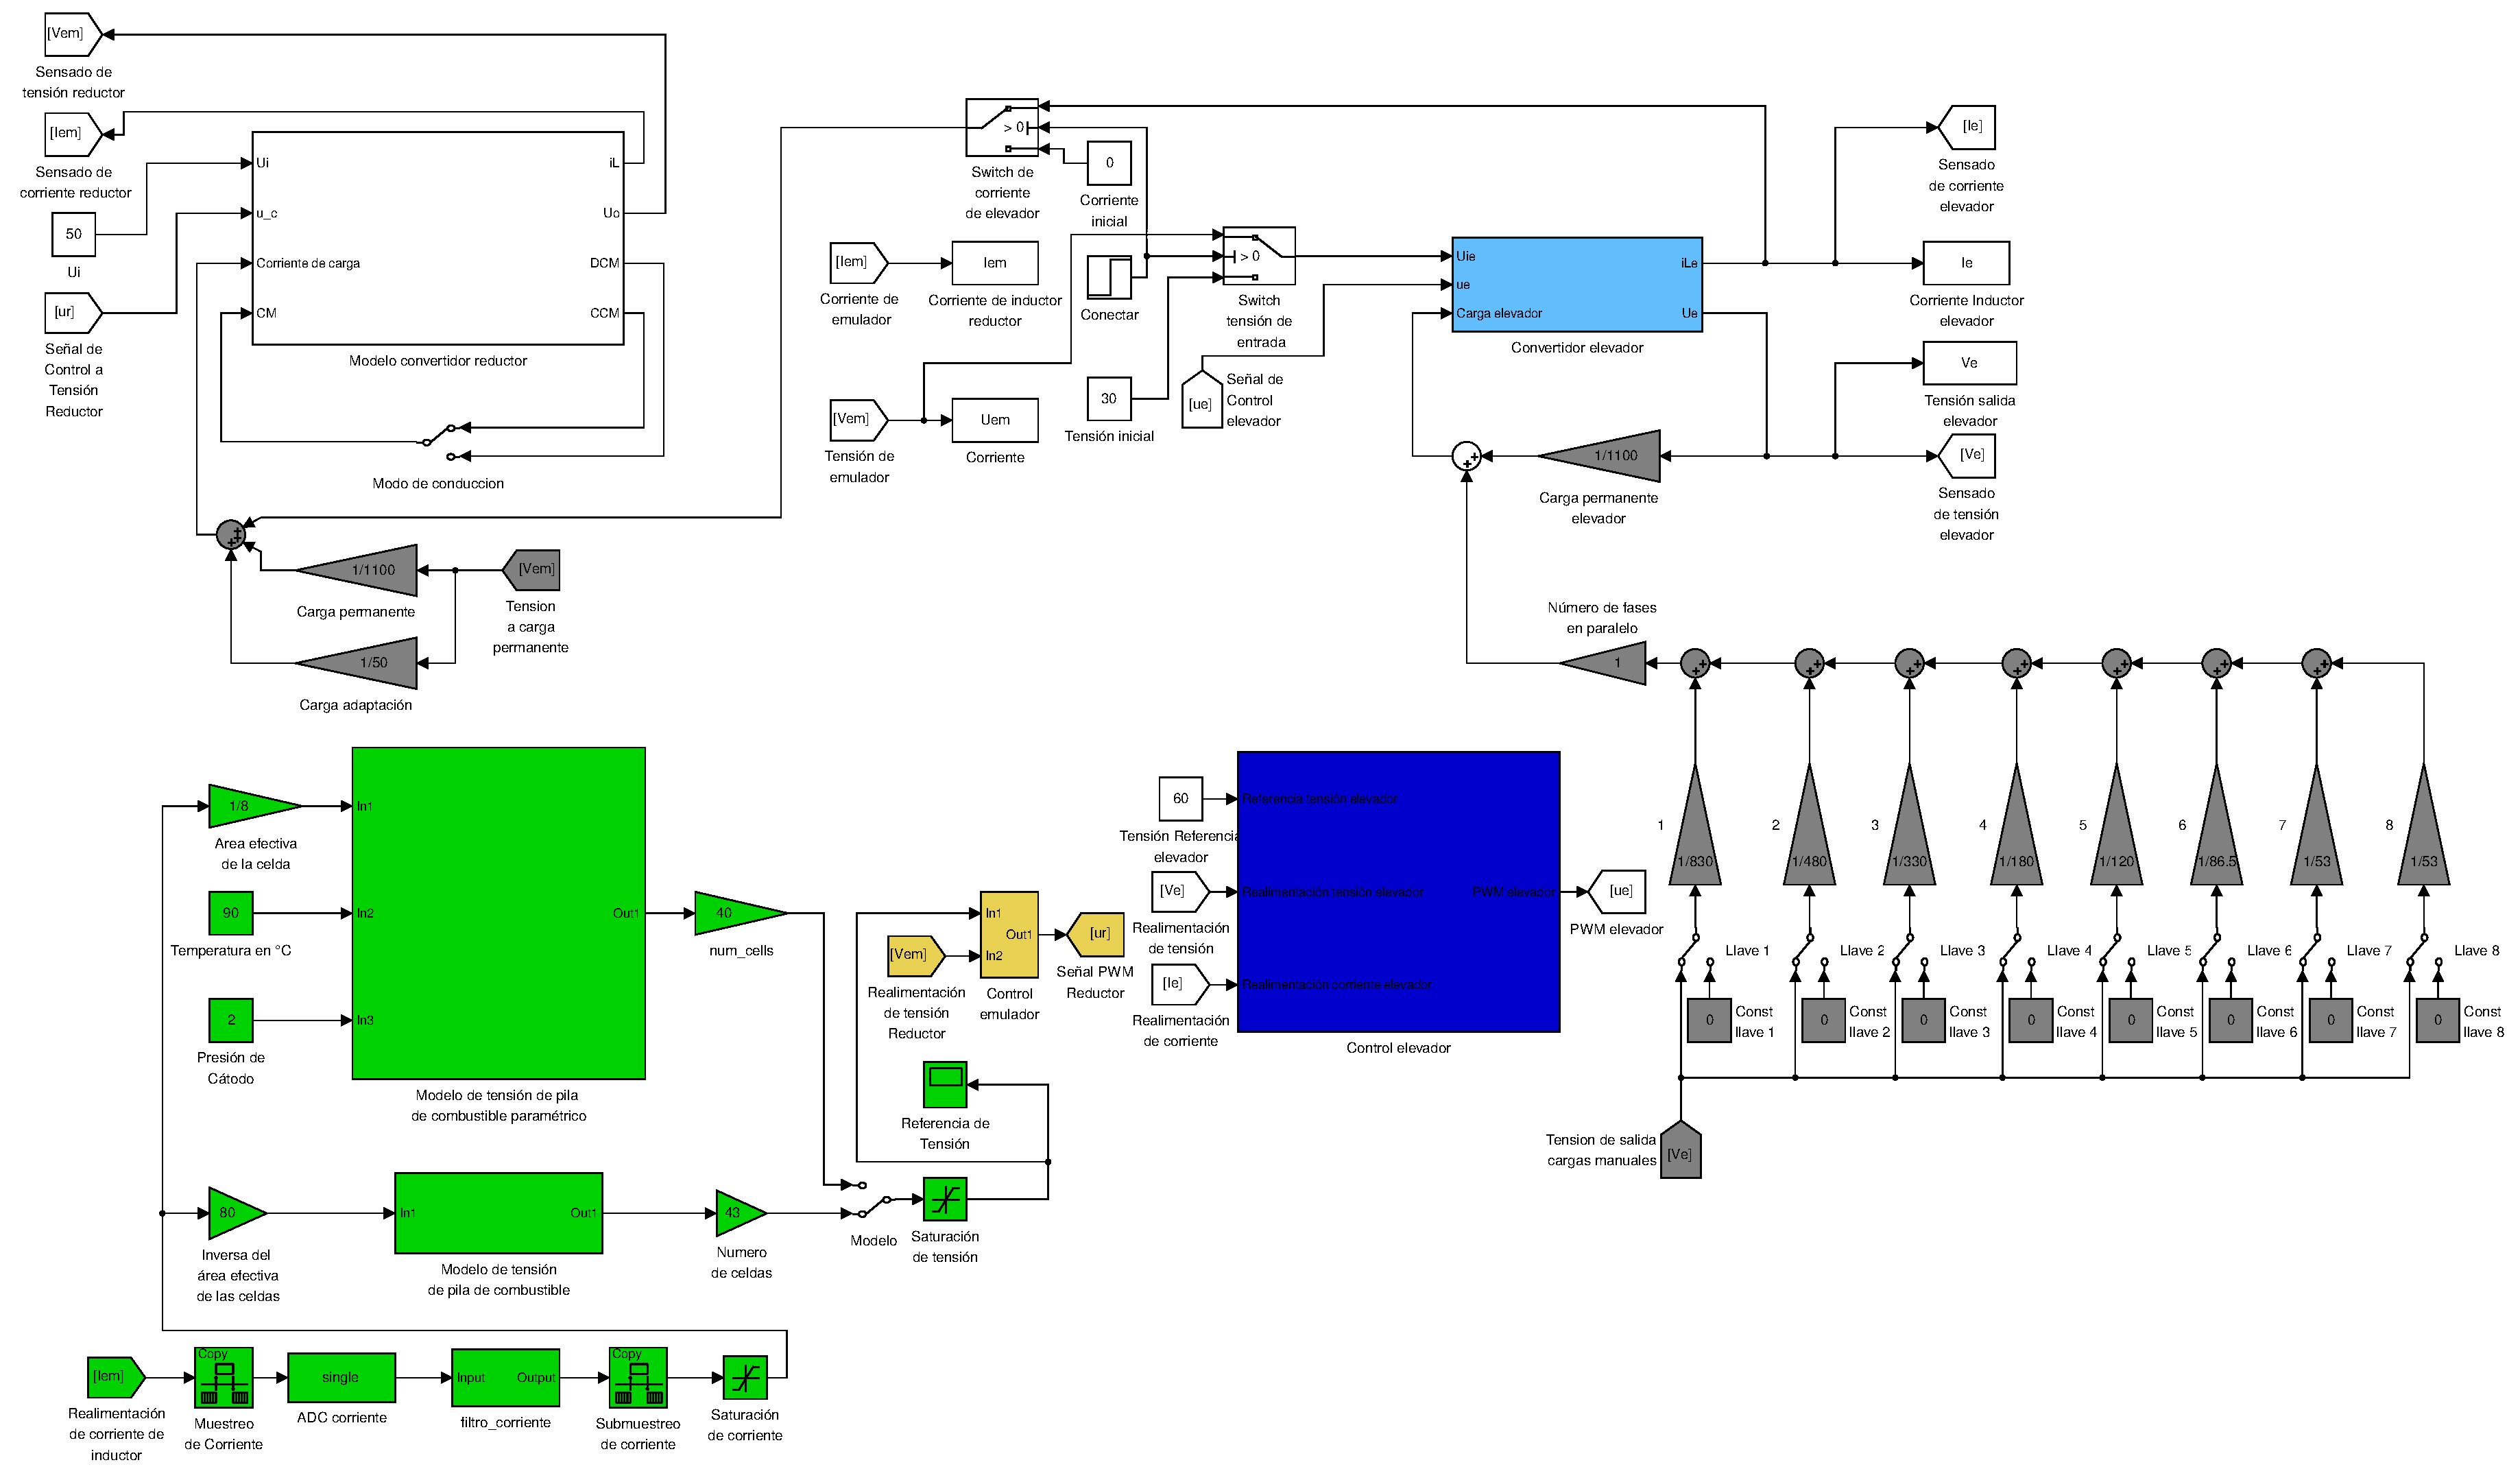
\includegraphics[width=11cm]{gfx/modelo_emulador_acoplado.eps}
 \caption{Esquema del emulador conectado a la etapa de potencia}
 \label{fig:modelo_emulador_acoplado}
\end{figure}

\begin{figure}[H]
 \centering
 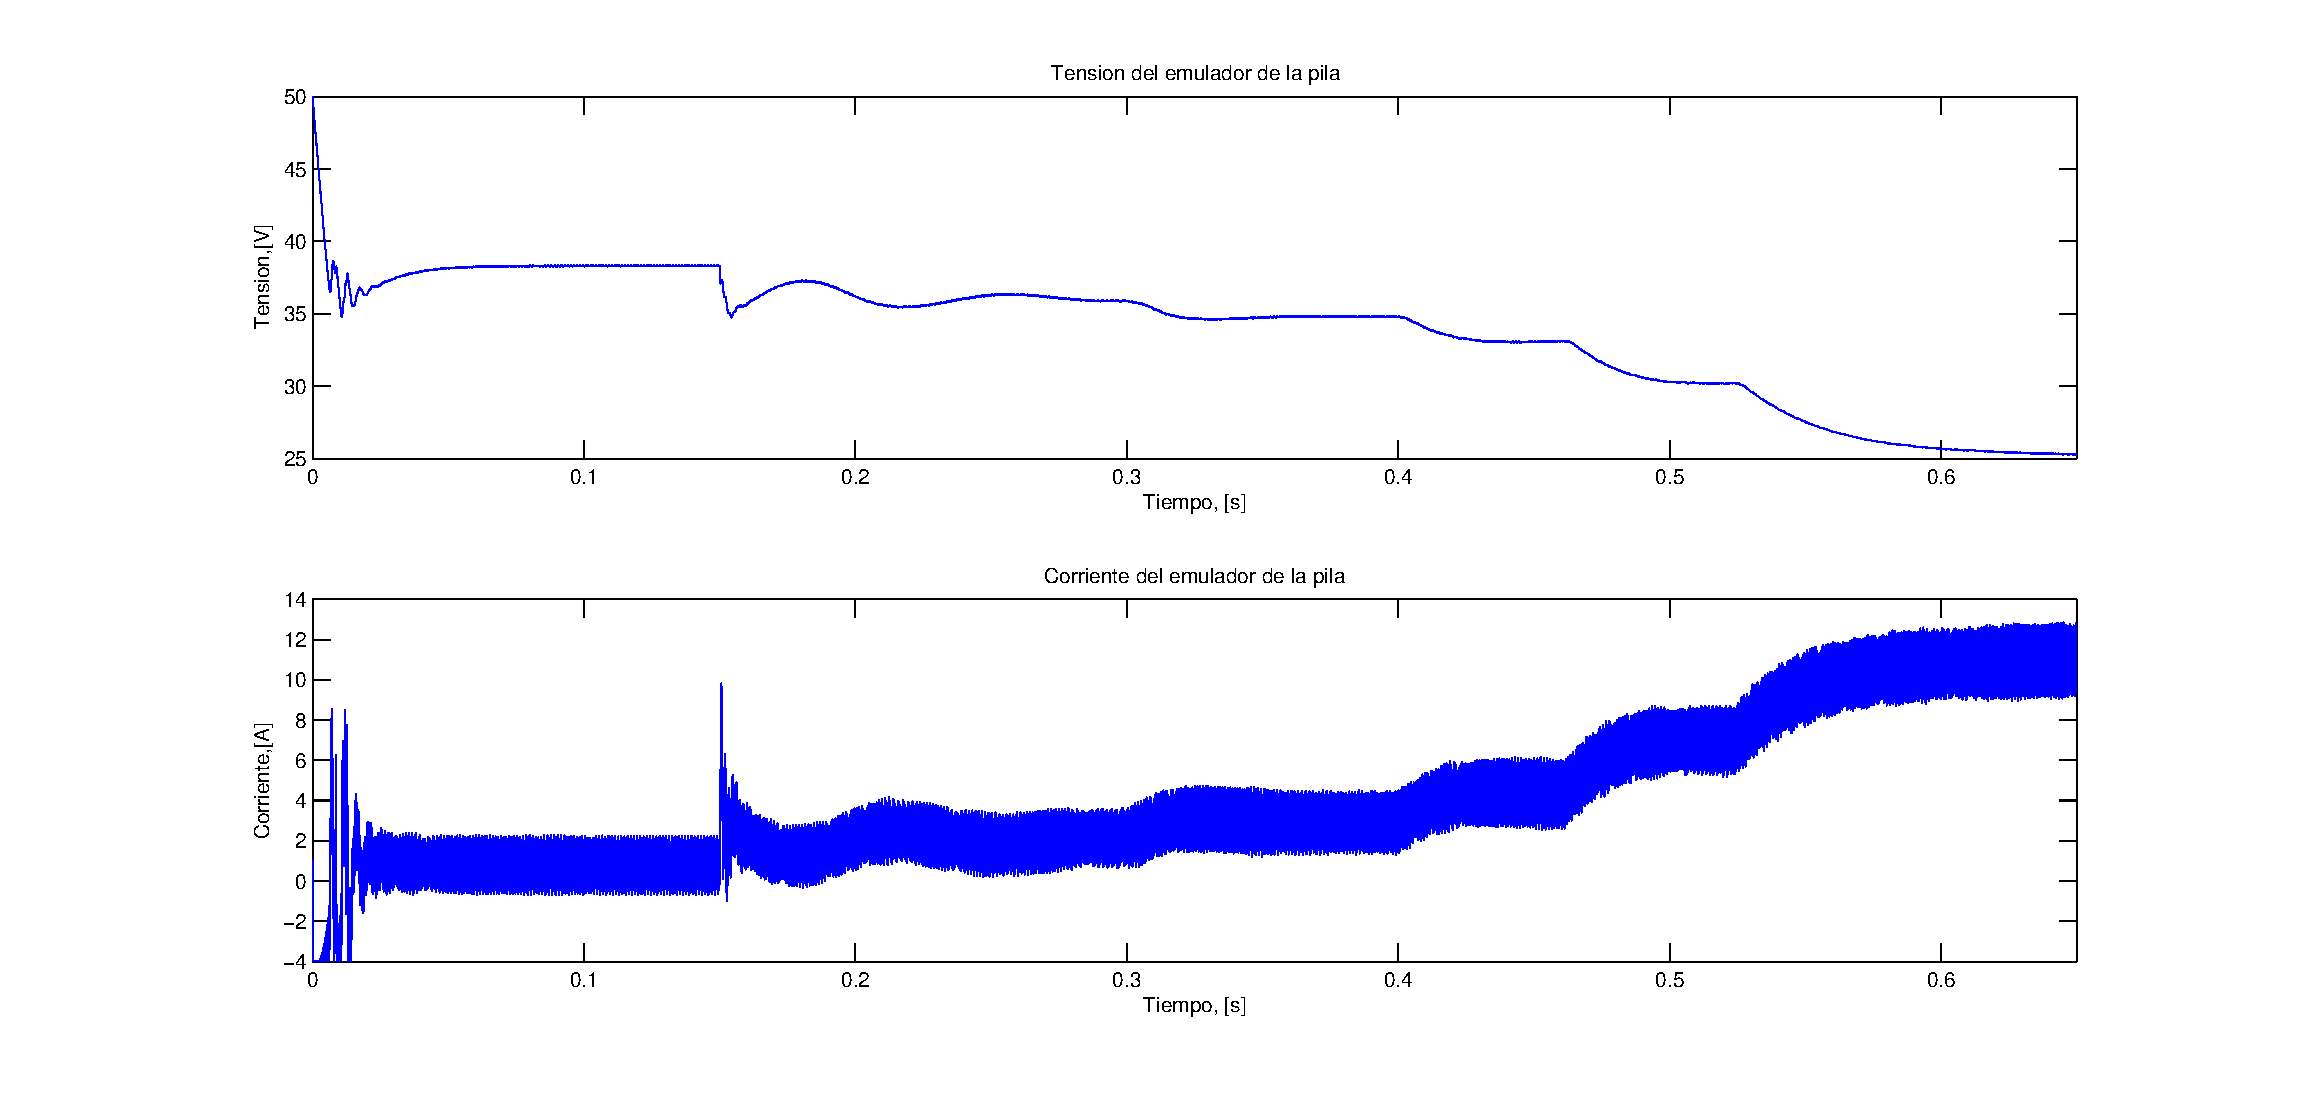
\includegraphics[width=11cm]{gfx/curvas_emulador_acoplado.eps}
 \caption{Esquema del emulador conectado a la etapa de potencia}
 \label{fig:curvas_emulador_acoplado}
\end{figure}

\begin{figure}[H]
 \centering
 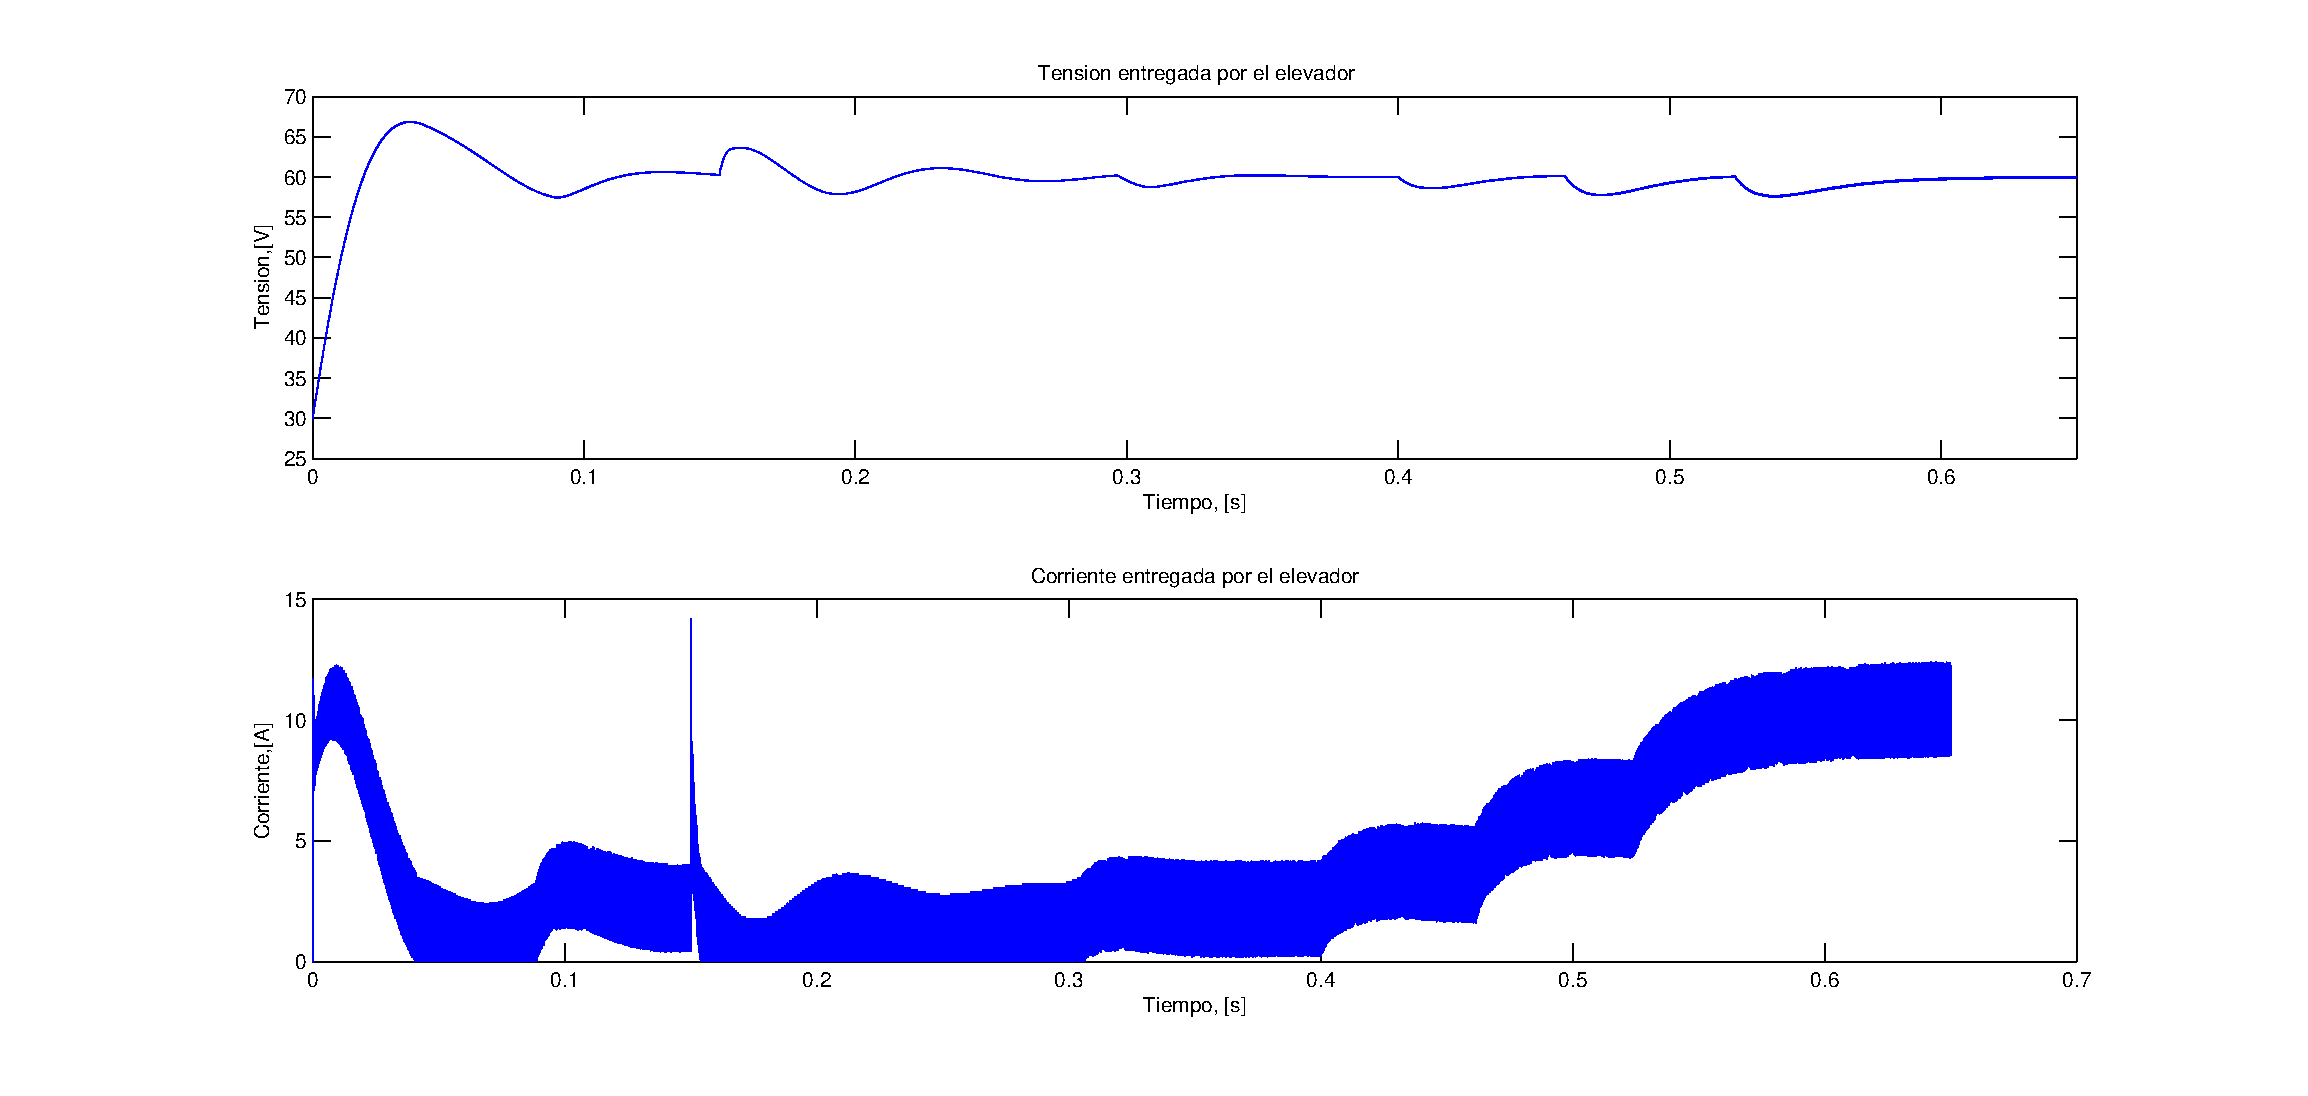
\includegraphics[width=11cm]{gfx/curvas_elevador_acoplado.eps}
 \caption{Esquema del emulador conectado a la etapa de potencia}
 \label{fig:curvas_elevador_acoplado}
\end{figure}


\subsection{Comentarios}
Los resultados de simulación coinciden con los que se esperaban, por lo tanto los modelos utilizados son válidos y se procedió al ensayo
de los convertidores y la evaluación del emulador en el laboratorio, cuyos resultados se presentan en el capitulo siguiente.
\end{document}
\end{comment}
